%!TEX root = ../template.tex
%%%%%%%%%%%%%%%%%%%%%%%%%%%%%%%%%%%%%%%%%%%%%%%%%%%%%%%%%%%%%%%%%%%%
%% 4-Work_Done.tex
%% NOVA thesis document file
%%
%% Chapter with the template manual
%%%%%%%%%%%%%%%%%%%%%%%%%%%%%%%%%%%%%%%%%%%%%%%%%%%%%%%%%%%%%%%%%%%%

\typeout{NT FILE 4-Centralized_Development.tex}%

\chapter{Centralized Development}
\label{cha:Centralized Development}

\glsresetall

\section{Introduction} \label{sec.4:Introduction}
As discussed in Section~\ref{cha:State of the art}, most existing methods for agent separation and encirclement operate either in \gls{2D} or \gls{3D}. This chapter focuses on a method that is believed to differ from those previously presented for \gls{3D} formations. While it builds upon them as a basis and source of inspiration, it introduces a novel approach to separation on the two-sphere.

This chapter is structured into two principal components. The first concerns methods for distributing points on the two-sphere (Section~\ref{sec.4:Comparison of Agent Distributions on the Two-Sphere}), addressing how the desired final positions of a given number of agents can be arranged over the sphere. The second component presents the chosen control architecture (Section~\ref{sec.4:Control loop architecture} responsible for tracking and encircling the target).

Since spherical projections are used repeatedly throughout the analysis, the operator $\Pi_{\Gamma^2}^{R,P}(\cdot)$ is defined to denote the projection onto a sphere of radius $R$ located at $P$, being for example $\Pi_{\Gamma^2}^{1,0}$ the unit sphere at the origin. This operator is defined as $\Pi_{\Gamma^2}^{R,P} : \mathbb{R}^3 \to \Gamma^2(R,P)$ 
\begin{equation}
\Pi_{\Gamma^2}^{R,P}(p)
\;=\;
P + R \frac{p - P}{\|p - P\|},
\qquad p \neq P,
\label{eq:sphere_projections}
\end{equation}
where $\Gamma^2(R,P)$ denotes the two-sphere of radius $R > 0$ centered at $P \in \mathbb{R}^3$, as defined above. The points $\gls{q_i}, \gls{q_i_desired} \in \Gamma^2$ are defined as 
\begin{equation}
    \gls{q_i} = \Pi_{\Gamma^2}^{\gls{ith_sphere_radius},\gls{target_pos}}(\gls{chaser_i_pos}) \;,\quad \gls{q_i_desired} = \Pi_{\Gamma^2}^{\gls{ith_sphere_radius},\gls{target_pos}}(\gls{p_i_desired})
    \label{eq:projections_q_and_p}
\end{equation}
are the projection of the drone $i$ to the current sphere of radius \gls{ith_sphere_radius} located around the target and the projection of desired final position points projected on the current radius \gls{ith_sphere_radius} also located around the target \gls{target_pos} respectively.

\section{Comparison of Agent Distributions on the Two-Sphere} \label{sec.4:Comparison of Agent Distributions on the Two-Sphere}

As outlined in Section~\ref{sec.3:Direct computation agent spacing on the two-sphere}, multiple approaches exist for distributing a prescribed number of agents on the two-sphere. Since the number of agents is predefined and the position of all agents is known by all agents, direct computation methods can and are used in this section, the outcomes of each method are presented and systematically compared. Based on this comparison, the most suitable centralized method is identified in light of the objectives and constraints of the present study.

\begin{figure}[htbp]
\centering

\begin{minipage}{0.12\textwidth} % width for the row label
Latitude \&\\Longitude:
\end{minipage}%
\begin{minipage}{0.85\textwidth} % width for the row of sub figures
\subfloat[Normal]{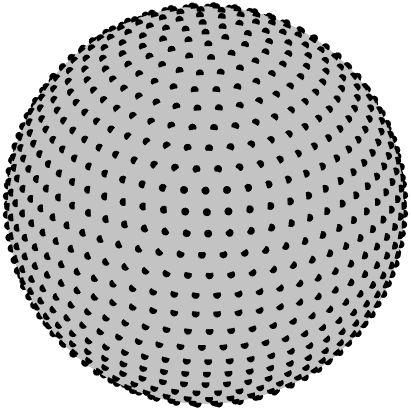
\includegraphics[width=3cm]{5-Figures/Chapter4/latlon_sphere/latlon_sphere_normal.png}}\hfil
\subfloat[Top]{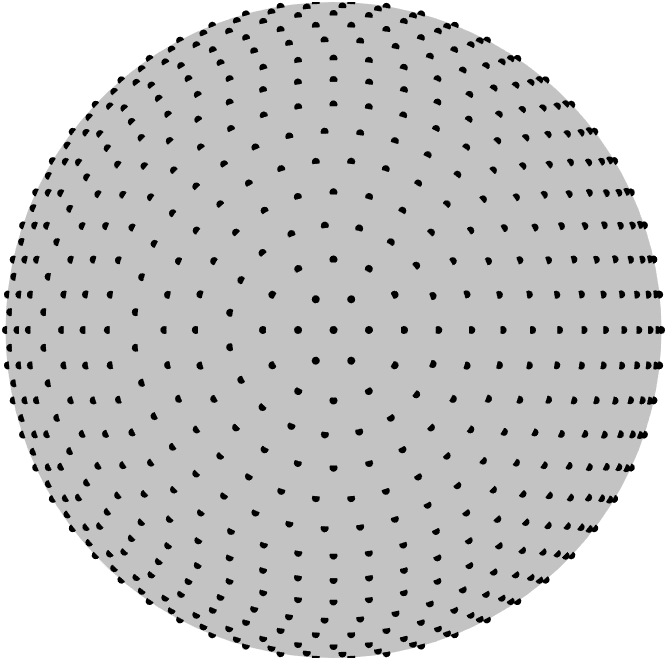
\includegraphics[width=3cm]{5-Figures/Chapter4/latlon_sphere/latlon_sphere_top.png}}\hfil 
\subfloat[Side]{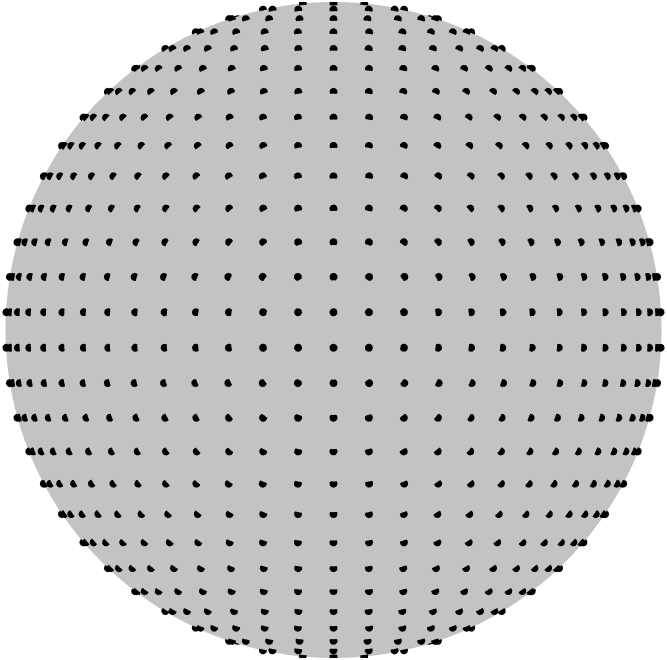
\includegraphics[width=3cm]{5-Figures/Chapter4/latlon_sphere/latlon_sphere_side.png}}
\end{minipage}

\vspace{0.3cm}

\begin{minipage}{0.12\textwidth}
Fibonacci\\Lattice:
\end{minipage}%
\begin{minipage}{0.85\textwidth}
\subfloat[Normal]{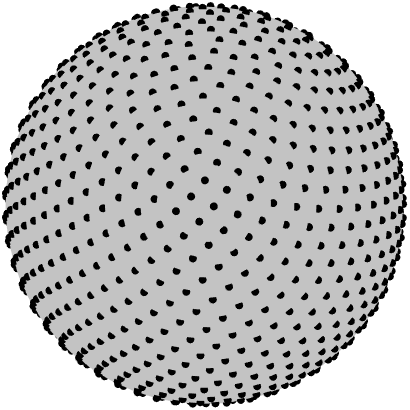
\includegraphics[width=3cm]{5-Figures/Chapter4/fibonacci_sphere/fibonacci_sphere_normal.png}}\hfil   
\subfloat[Top]{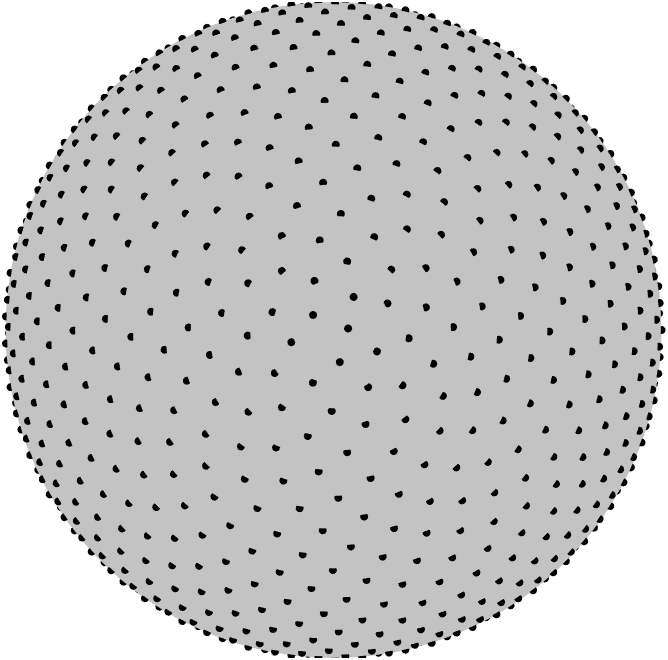
\includegraphics[width=3cm]{5-Figures/Chapter4/fibonacci_sphere/fibonacci_sphere_top.png}}\hfil
\subfloat[Side]{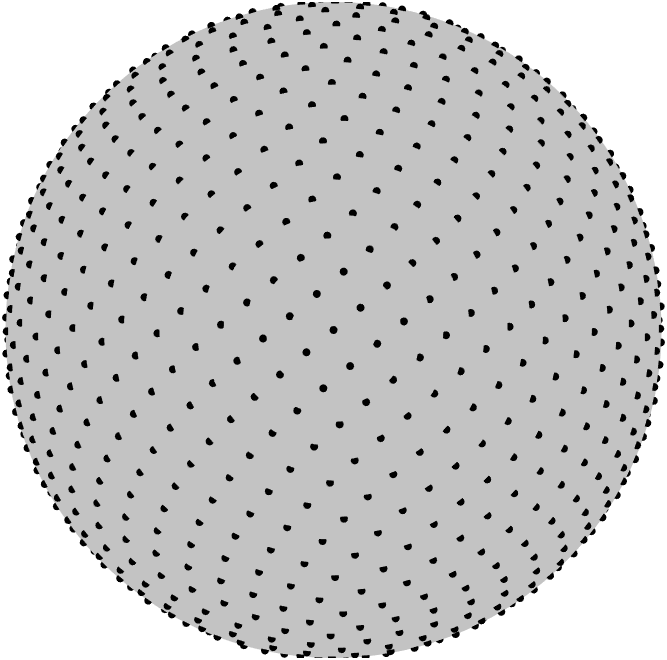
\includegraphics[width=3cm]{5-Figures/Chapter4/fibonacci_sphere/fibonacci_sphere_side.png}}
\end{minipage}

\vspace{0.3cm}

\begin{minipage}{0.12\textwidth}
Poisson Disk\\Sampling:
\end{minipage}%
\begin{minipage}{0.85\textwidth}
\subfloat[Normal]{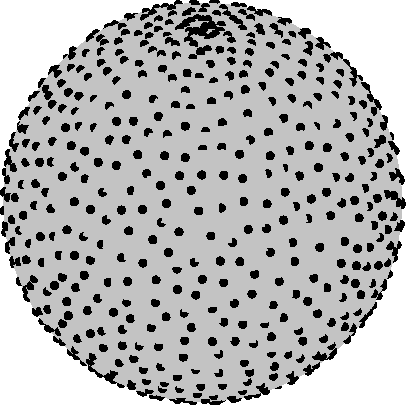
\includegraphics[width=3cm]{5-Figures/Chapter3/poisson_disk/poisson_disk_normal.pdf}}\hfil   
\subfloat[Top]{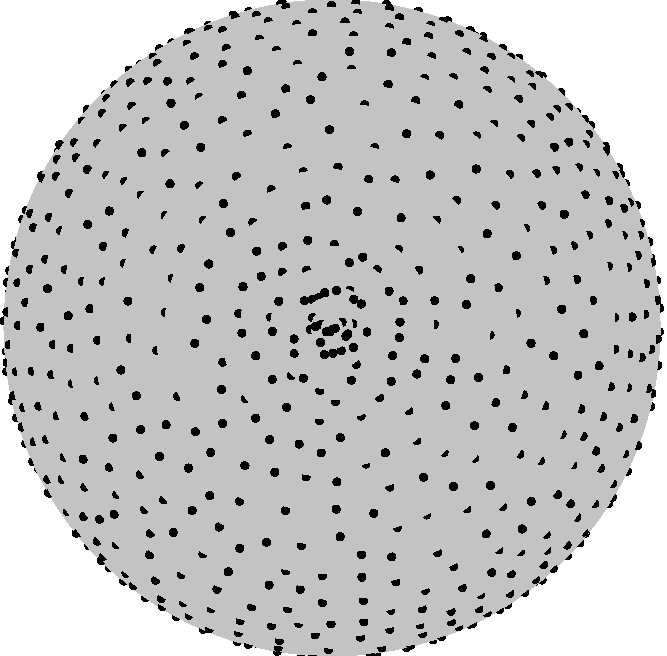
\includegraphics[width=3cm]{5-Figures/Chapter3/poisson_disk/poisson_disk_top.pdf}}\hfil
\subfloat[Side]{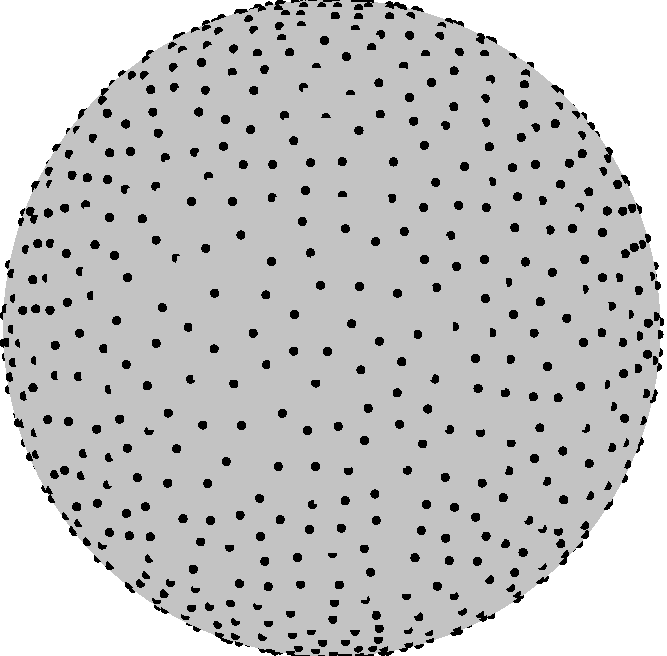
\includegraphics[width=3cm]{5-Figures/Chapter3/poisson_disk/poisson_disk_side.pdf}}
\end{minipage}

\caption{Agent positions resulting from each distribution methods.}
\label{fig.4:centalized_methods_points_on_sphere}
\end{figure}

\begin{figure}[htbp]
  \centering
  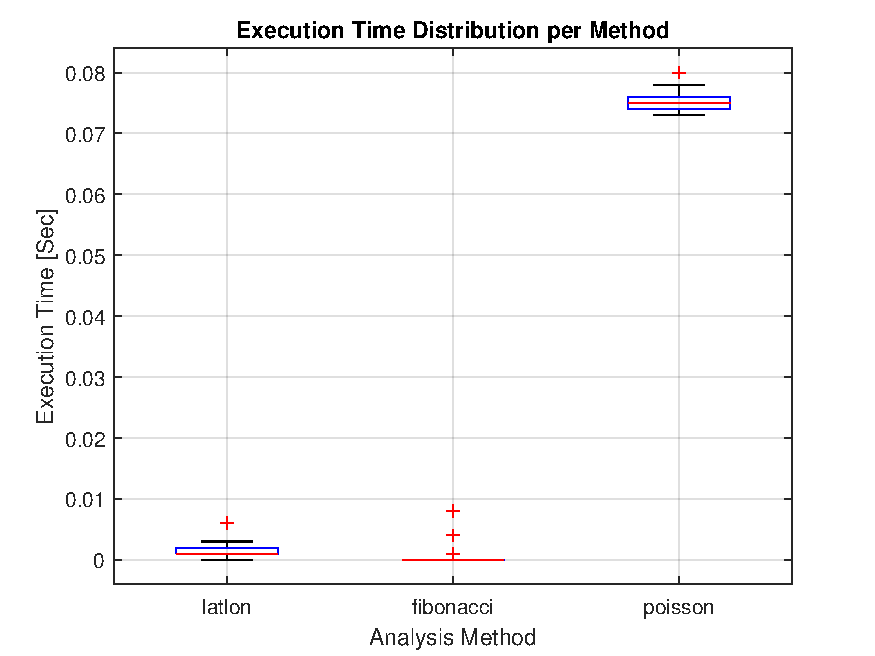
\includegraphics[width=0.85\textwidth]{5-Figures/Chapter4/centralized_comparing_methods_box_shape.pdf}
  \caption{Overall runtime comparison of the different methods (100 trials). Computer specification can be found at: \ref{appendix:Computer Specifications}}
  \label{fig.4:centalized_comparing_methods_box_shape}
\end{figure}

As shown in Figures~\ref{fig.4:centalized_methods_points_on_sphere}, the three methods produce noticeably different agent distributions. The longitude \& latitude method can be discarded due to limitation of number of agent formations possible, in case of the lost of one agent a new formation would not be possible. This leaves two viable options: the Fibonacci lattice and Poisson disk sampling. The Fibonacci lattice is the fastest of the two methods as shown in Figure~\ref{fig.4:centalized_comparing_methods_box_shape} being still $666.66\dots\%$ faster on average while providing uniform coverage, but it is restricted to distributions on a spherical surface and is less flexible for arbitrary domains. Poisson disk sampling, in contrast, is more versatile and can be applied to arbitrary geometries, but it requires more computation and a gradient-based refinement step to achieve a fixed number of agents being the necessary separation distance initially unknown. Each method thus presents a trade-off between computational efficiency, uniformity, and flexibility. Due to the simplicity of the Fibonacci Lattice, it was chosen as the preferred distribution method for centralized systems.

\begin{table}[htbp]
\caption{Runtime comparison of point sampling methods}
\label{tab.4:Runtime comparison of point sampling methods}
\centering
\begin{tabular}{l c c c c}
\hline
\textbf{Property}
& \makecell{\textbf{Lon--Lat}}
& \makecell{\textbf{Fibonacci}}
& \makecell{\textbf{Poisson Disk}} \\
\hline
\makecell{Parameters}
& \makecell{$K=29$}
& \makecell{--}
& \makecell{$k = 30$,\\ $r=0.093$} \\

\makecell{Number of points}
& \makecell{1070}
& \makecell{1001}
& \makecell{1028} \\

\makecell{Mean runtime\\ (s)}
& \makecell{0.0016}
& \makecell{$2.4\times10^{-4}$}
& \makecell{0.0751} \\

\makecell{Std. deviation\\ $\sigma$ (s)}
& \makecell{$7.6877\times10^{-4}$}
& \makecell{$9.3333\times10^{-4}$}
& \makecell{0.0014} \\
\hline
\end{tabular}
\end{table}

\section{Alternative Agent Positioning Strategies} \label{sec.4:Alternative Agent Positioning Strategies}

This section discusses alternative methods that were considered to work to position agents on a spherical surface. Although the final configuration of each drone is based on the Fibonacci lattice, several other approaches were investigated, inspired by phase-separation methods commonly used for 2D formations \cite{Litimein2021}, \cite{Jin2018}, \cite{Kim2007}.  In particular, an attempt was made to develop a displacement-based 3D method in which each drone maintains a fixed angular separation from its predecessor.

The standard Fibonacci lattice formulation could not be directly applied in this context. While the longitude increments between agents are constant, allowing a simple angular separation rule, the latitude is computed through a nonlinear $\arcsin(\cdot)$ mapping, which is inherently non-uniform. This nonlinearity prevents the use of a single, constant spacing rule across all agents. Several attempts were made to linearize this relationship so that all agents could rely on identical local control laws, but none yielded satisfactory results. For completeness, the tested approaches are summarized below.

\subsection{Mean Distance Between Points on the Sphere}
In the first attempt, the geodesic distance between consecutive agents in the sequence was computed, and the mean of these distances was used as a reference spacing. This approach proved unsuccessful, as illustrated in Figure~\ref{fig.4:fibonacci_diff_methods} (row~2). The mean distance is heavily skewed by agents located near $\theta = \pi$, where inter-agent distances are significantly larger. For example, with 1001 points distributed on a sphere of radius $R = 5$, the mean distance was approximately 7.3270, corresponding to more than half the sphere's diameter. As a result, this metric does not provide a meaningful or usable spacing reference.

\subsection{Mean Latitude Spacing}
Since the primary source of nonlinearity lies in the latitude distribution, a second approach considered using the average latitude increment instead of the $\arcsin(\cdot)$ mapping. However, this method introduces a different issue: the geodesic distance between agents increases as the effective radius of the latitude circle grows, particularly near $\theta = \pi$. This results in a pronounced clustering of points near longitudes $\phi = 0$ and $\phi = 2\pi$, as shown in Figure~\ref{fig.4:fibonacci_diff_methods} (row~3). While the $\arcsin(\cdot)$ formulation avoids this clustering, the mean-latitude approach fails to preserve uniform surface spacing.

\subsection{Linearized Vertical Distribution with Uniform Angular Progression}
A final attempt aimed to mitigate the clustering near the poles by enforcing a uniform angular progression while simultaneously liberalizing the vertical distribution. Instead of relying on the nonlinear Fibonacci latitude mapping, a constant latitude increment $\theta_{\text{mean}} = \pi / P$ was imposed. In parallel, a constant longitude increment $\phi_{\text{mean}}$ was computed from the average difference of the Fibonacci-based longitudes.

The Cartesian coordinates of each agent were defined as
\begin{equation}
x_i = R \sin(i\theta_{\text{mean}})\cos(i\phi_{\text{mean}}), \quad
y_i = R \sin(i\theta_{\text{mean}})\sin(i\phi_{\text{mean}}),
\end{equation}
with the vertical coordinate distributed linearly according to
\begin{equation}
z_i = -R + \frac{R}{P} + \frac{2R(i-1)}{P},
\end{equation}
thereby enforcing equal spacing along the $z$-axis.

The motivation for this approach was twofold. First, by fixing $\theta_{\text{mean}}$, each agent would only need to maintain a constant angular separation from its predecessor. Second, by distributing agents uniformly along the vertical axis, the excessive clustering near the poles observed in previous methods could be reduced. As shown in Figure~\ref{fig.4:fibonacci_diff_methods} (row~4), this method successfully eliminates severe polar clustering and yields a visually more homogeneous vertical distribution.

However, despite these improvements, this approach still fails to guarantee uniform geodesic distances between neighboring agents. The imposed linearity in both $\theta$ and $z$ conflicts with the intrinsic geometry of the sphere, resulting in distorted inter-agent spacing. In particular, agents near the north and south region become closer than desired. The resulting shape comes due to the fact the points are forced (as intended) to spread equally along the z axis but this in turn makes the $i^{th}$ element be much lower than would be expected by X and Y coordinates.

\begin{figure}[htbp]
\centering

\begin{minipage}{0.12\textwidth}
Fibonacci\\Lattice:
\end{minipage}%
\begin{minipage}{0.85\textwidth}
\subfloat[Normal]{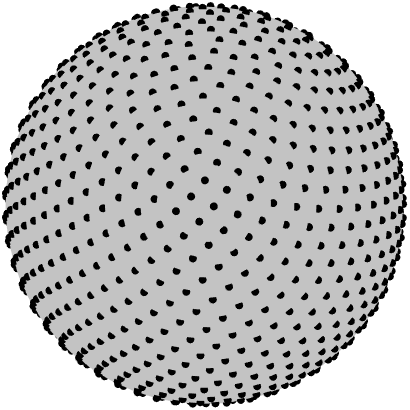
\includegraphics[width=3cm]{5-Figures/Chapter4/fibonacci_sphere/fibonacci_sphere_normal.png}}\hfil   
\subfloat[Top]{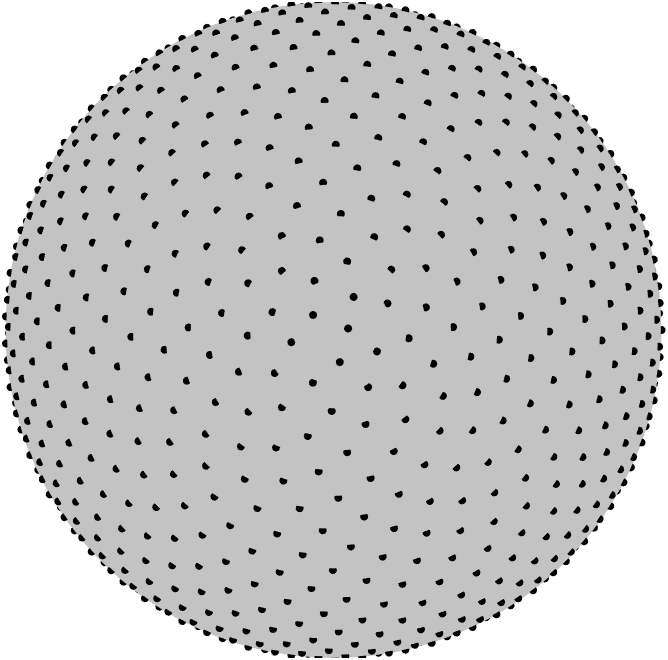
\includegraphics[width=3cm]{5-Figures/Chapter4/fibonacci_sphere/fibonacci_sphere_top.png}}\hfil
\subfloat[Side]{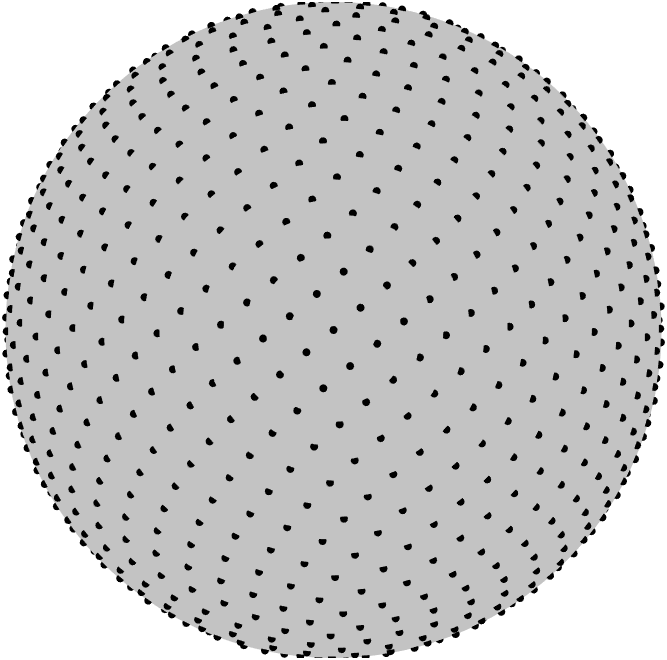
\includegraphics[width=3cm]{5-Figures/Chapter4/fibonacci_sphere/fibonacci_sphere_side.png}}
\end{minipage}

\vspace{0.3cm}

\begin{minipage}{0.12\textwidth}
mean\\dist:
\end{minipage}%
\begin{minipage}{0.85\textwidth}
\subfloat[Normal]{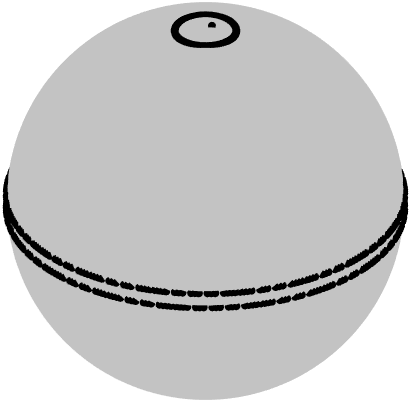
\includegraphics[width=3cm]{5-Figures/Chapter4/fibonacci_sphere_mean_dist/fibonacci_sphere_mean_dist_normal.png}}\hfil   
\subfloat[Top]{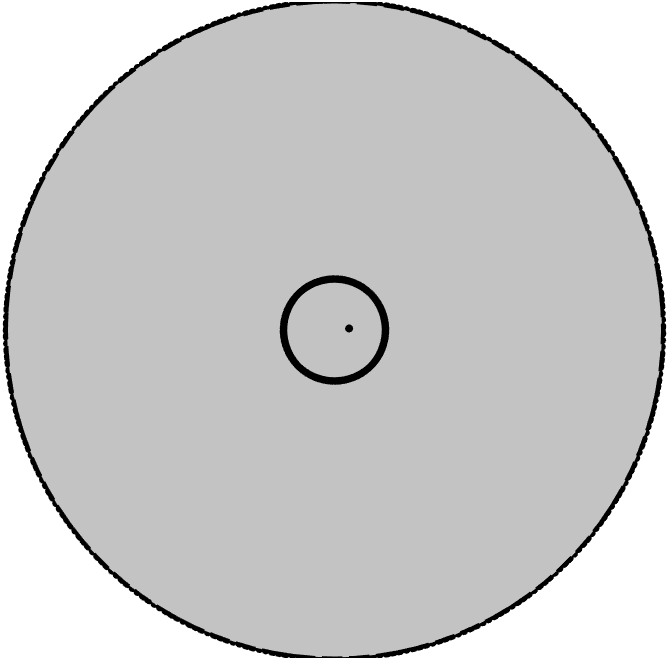
\includegraphics[width=3cm]{5-Figures/Chapter4/fibonacci_sphere_mean_dist/fibonacci_sphere_mean_dist_top.png}}\hfil
\subfloat[Side]{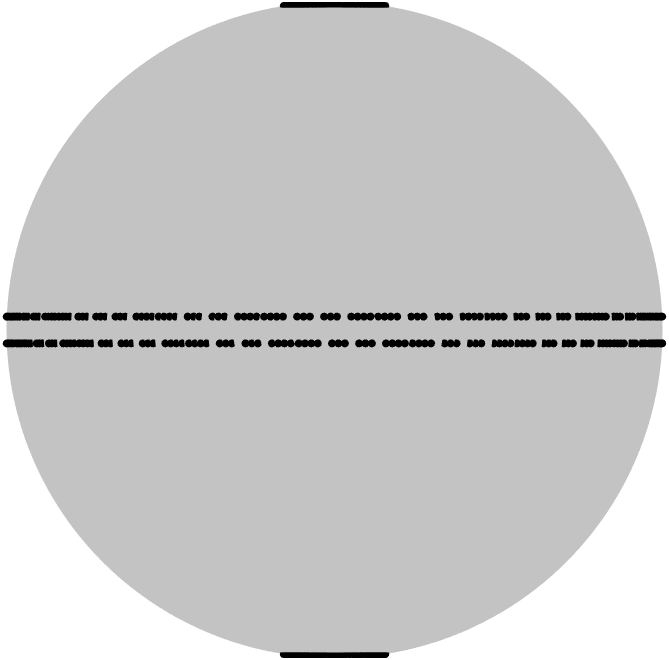
\includegraphics[width=3cm]{5-Figures/Chapter4/fibonacci_sphere_mean_dist/fibonacci_sphere_mean_dist_side.png}}
\end{minipage}

\vspace{0.3cm}

\begin{minipage}{0.12\textwidth}
mean theta:
\end{minipage}%
\begin{minipage}{0.85\textwidth}
\subfloat[Normal]{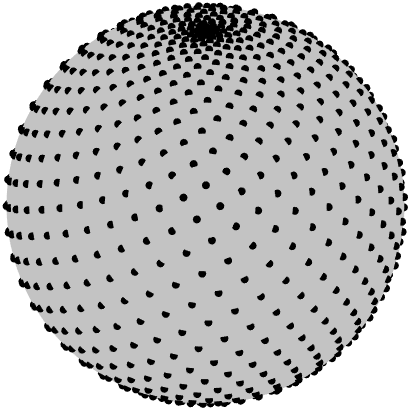
\includegraphics[width=3cm]{5-Figures/Chapter4/fibonacci_sphere_mean_theta/fibonacci_sphere_mean_theta_normal.png}}\hfil   
\subfloat[Top]{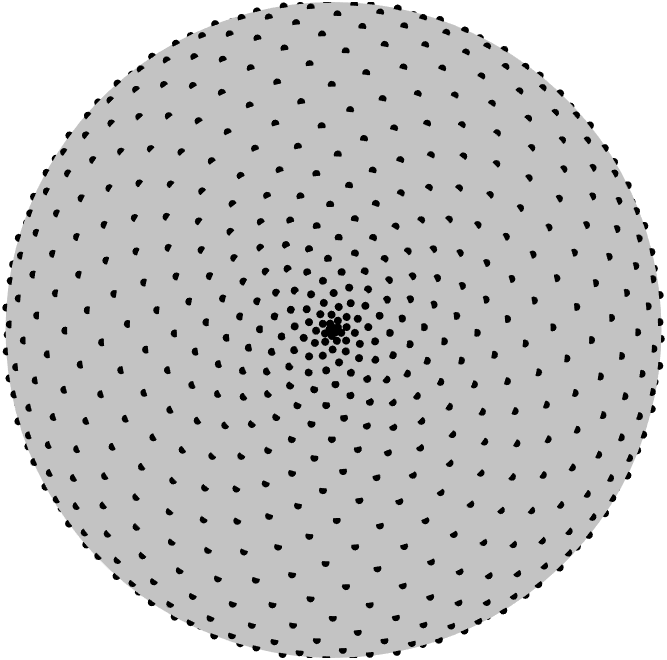
\includegraphics[width=3cm]{5-Figures/Chapter4/fibonacci_sphere_mean_theta/fibonacci_sphere_mean_theta_top.png}}\hfil
\subfloat[Side]{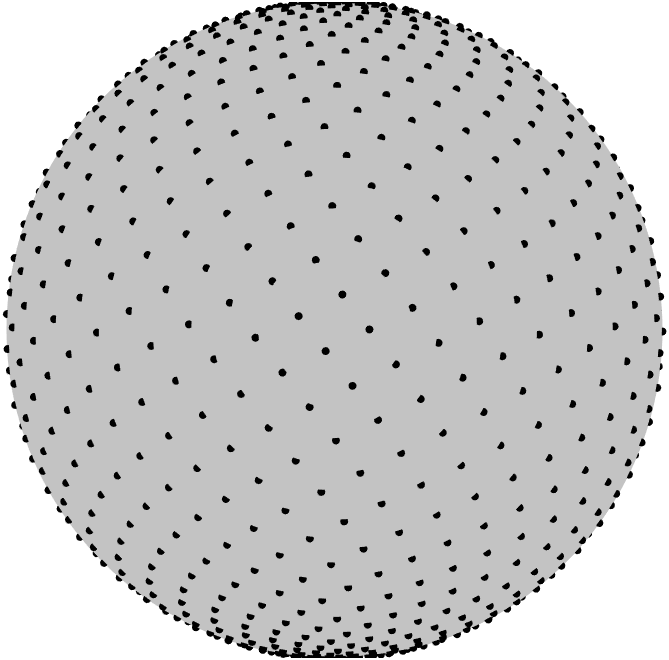
\includegraphics[width=3cm]{5-Figures/Chapter4/fibonacci_sphere_mean_theta/fibonacci_sphere_mean_theta_side.png}}
\end{minipage}

\vspace{0.3cm}
\begin{minipage}{0.12\textwidth}
mean theta\\eq z:
\end{minipage}%
\begin{minipage}{0.85\textwidth}
\subfloat[Normal]{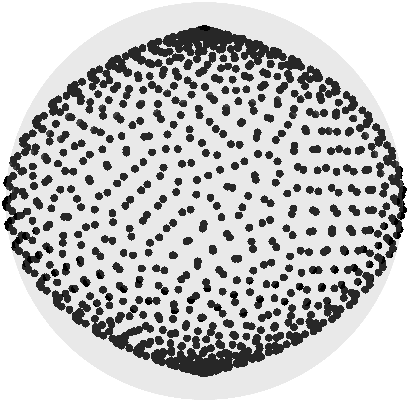
\includegraphics[width=3cm]{5-Figures/Chapter4/fibonacci_sphere_mean_theta_eq_z/fibonacci_sphere_mean_theta_eq_z_normal.png}}\hfil   
\subfloat[Top]{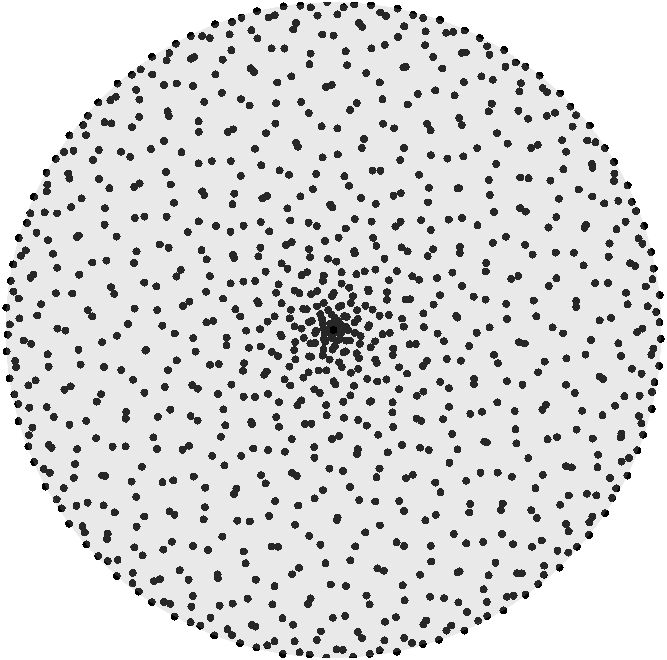
\includegraphics[width=3cm]{5-Figures/Chapter4/fibonacci_sphere_mean_theta_eq_z/fibonacci_sphere_mean_theta_eq_z_top.png}}\hfil
\subfloat[Side]{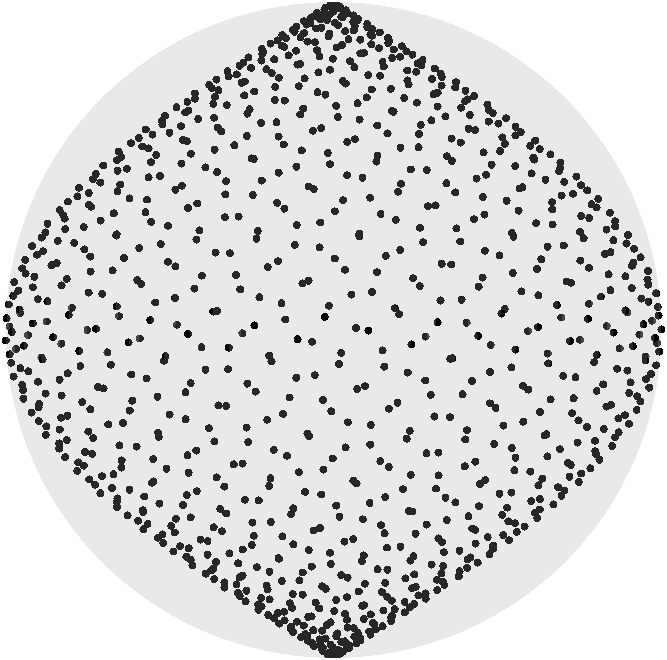
\includegraphics[width=3cm]{5-Figures/Chapter4/fibonacci_sphere_mean_theta_eq_z/fibonacci_sphere_mean_theta_eq_z_side.png}}
\end{minipage}
\caption{Different linearization of fibonacci lattice}
\label{fig.4:fibonacci_diff_methods}
\end{figure}

In summary, while this final approach partially alleviates the pole-clustering problem and simplifies the local control law by enforcing constant angular steps, it does so at the cost of losing the equal-area and near-uniform spacing properties of the standard Fibonacci lattice. As a result, it was ultimately deemed unsuitable for the final deployment strategy, but is included here for completeness and comparison with the other attempted methods. Either way this approach was flawed since opposite of the 2D approach where all drones are keeping a distance from the previous and next, in 3D the "top" and "bottom" drones aren't associated in any away.


\section{Control loop architecture} \label{sec.4:Control loop architecture}
This section describes the control strategy implemented for the drone, specifically a quadrotor, with the objective of not only reaching a desired position but also avoiding collisions with other agents. As mentioned in the introduction, the system is divided into multiple blocks, each responsible for a specific task.

Desired waypoints on the sphere are generated using the Fibonacci lattice, defining $\gls{p_desired}$. The Mellinger controller follows the reference $\gls{q}$ created by the geometric controller who is responsible for driving the quadrotor reference $\gls{q}$ toward the final desired point on the two-sphere, $\gls{q_desired}$. The radius controller reduces the distance between the chasers and the target until the desired radius, $\gls{desired_sphere_radius}$, is achieved.

Collision avoidance during motion is handled by an artificial potential field, which helps with safe separation between agents. Additionally, an exponential moving average combined with a consensus algorithm is used to estimate the position of the target.

The complete control architecture is illustrated in Figure~\ref{fig.4:controller_architecture}.

\begin{figure}
  \centering
  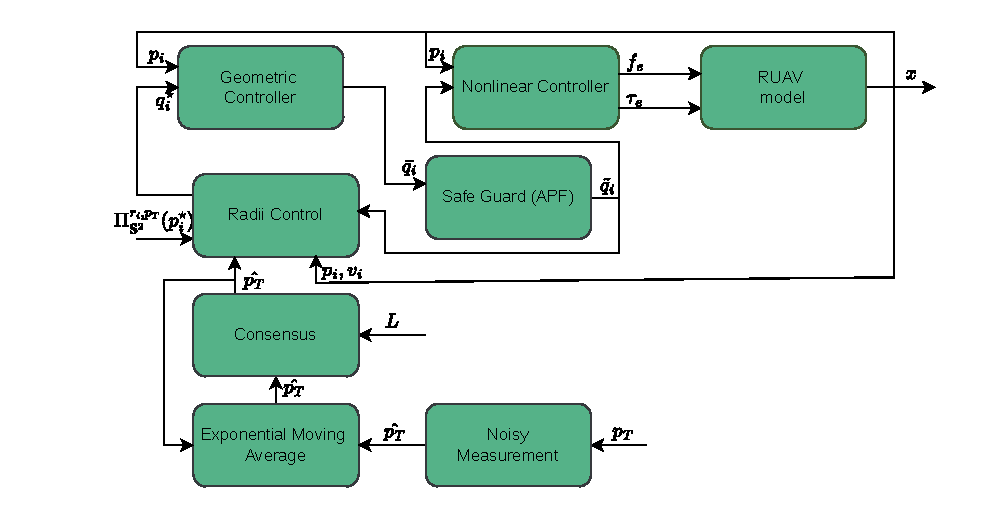
\includegraphics[width=\columnwidth]{5-Figures/Chapter4/controller_architecture/centralized_complete_controller_architecture.drawio.pdf}
  \caption{Controller architecture}
  \label{fig.4:controller_architecture}
\end{figure}

Before exploring the complete controller system the a simplified version of the problem will be studied where there only exists the drone controller and the geometric controller. This is due to the fact that multiple methods where studied for this controller and need to be compared without the influence of any other system variables/controllers. The inner loop is always fixed to a Mellinger controller since it has been proven to be effective, as shown in Figure~\ref{sec.3:Vehicle model and noninear control}. Two types of methodology will be shown either a desired inter distance of agents is given to the controller being then the controller a displacement based or simply the final desired position \gls{q_desired} if given, (position based). In both methods the initial position of the point on the sphere \gls{q} is the projection of the initial/current position of the drone on the two-sphere. Then this controller moves that point until a desired minimal distance \gls{min_dist} is met or the final desired position \gls{q_desired} is obtained. In Figures~\ref{fig.4:mellinger_controller_architecture} the inner--loop using a Mellinger controller can be seen while in Figure~\ref{fig.4:generelized_controller_architecture} the final controller can be seen where the controller in question for the outer--loop will be discussed, is one of the belows defined controllers. The variables \gls{p_desired} and \gls{q} both indicated desired drone position, \gls{v_desired} desired drone velocity and \gls{a_desired} desired drone accelerations.

\begin{figure}[htbp]
  \centering
  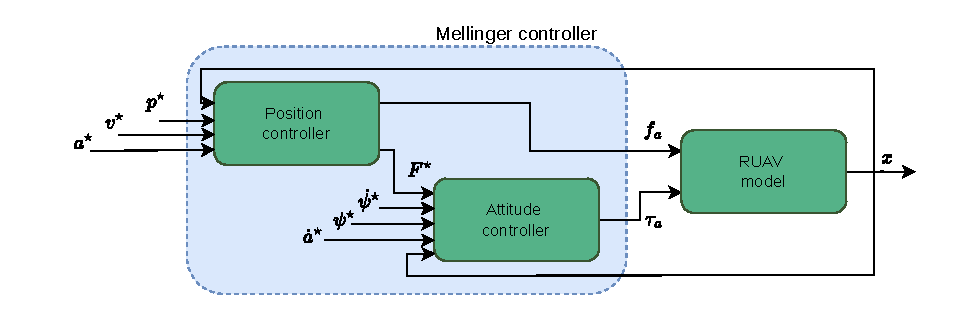
\includegraphics[width=\textwidth]{5-Figures/Chapter3/Mellinger Controller.pdf}
  \caption{NonLinear Controller architecture based in \cite{Mellinger2011}}
  \label{fig.4:mellinger_controller_architecture}
\end{figure}

\begin{figure}[htbp]
  \centering
  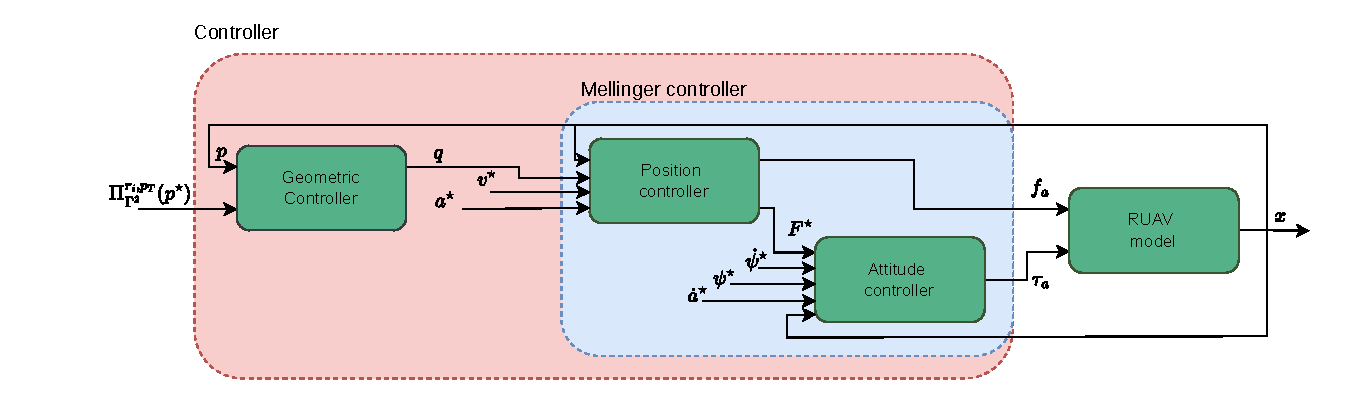
\includegraphics[width=\textwidth]{5-Figures/Chapter4/controller_architecture/simple_generalized_controller_architecture.pdf}
  \caption{outer/inner loop controller}
  \label{fig.4:generelized_controller_architecture}
\end{figure}

\subsection{Solvers (fmincon)}

The use of numerical solvers was investigated as a means of enforcing a minimum inter-agent distance while simultaneously guiding the drones toward a desired objective \gls{q_desired}, defined by Fibonacci lattice points on the sphere. The optimization problem was formulated with nonlinear constraints to ensure collision avoidance.

However, this approach suffers from a fundamental limitation: none of the verified solvers is capable of enforcing all nonlinear constraints at every timestep while also guaranteeing convergence to the desired objective. The nonlinear constraints are guaranteed to be satisfied only at the optimal solution, and not throughout the system's evolution.

Figure~\ref{fig.4:solver_solution} illustrates this issue for a scenario involving three drones. It can be observed that the intermediate solver-generated trajectories do not directly converge toward the Fibonacci lattice points, highlighting the practical limitations of this approach for real-time or tightly constrained multi-agent motion planning.

\begin{figure}[htbp]
  \centering
  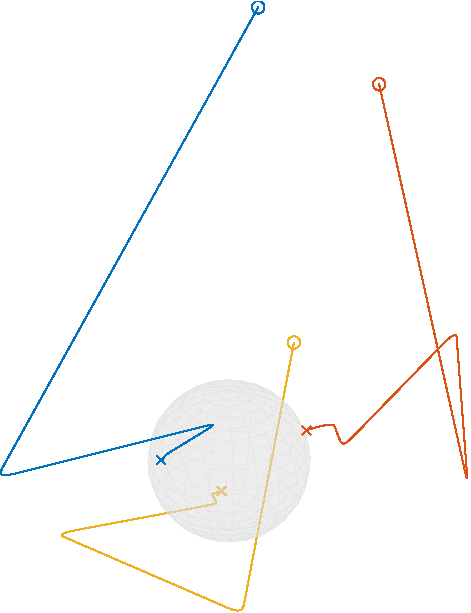
\includegraphics[width=0.4\textwidth]{5-Figures/Chapter4/solutions/solver.pdf}
  \caption{Trajectory obtained using an optimization-based solver (\texttt{fmincon}) for three drones.}
  \label{fig.4:solver_solution}
\end{figure}

\subsection{Artificial Potential Field (APF)}

The concept of \gls{APF} was previously introduced in
Section~\ref{sec.3:Artificial Potential Fields}. In this section, it is
applied to enforce inter-agent separation while maintaining a desired
spatial distribution on a spherical surface. Being the idea instead of guiding the points \gls{q} to their respective references the average distance between points is calculated from \gls{p_desired} in this case the Fibonacci Latices points and have the points \gls{q} spread until the same intra distance is obtained. Let \gls{n_D} denote the number of drones, and consider the set $\{ \gls{p_i_desired} \in \mathbb{S}^2 \}_{i=1}^{N_D}$ representing Fibonacci lattice points distributed on a sphere of radius \gls{desired_sphere_radius}. From this points the pairwise geodesic distance matrix $d_{ij}$ is computed according to
\begin{equation}
  d_{ij} =
  \begin{cases}
  r_s\arccos\!\left( \dfrac{\gls{q_i}^{\top}q_j}{\gls{desired_sphere_radius}^2} \right), & i \neq j, \\[6pt]
  \infty, & i = j ,
  \end{cases}
  \label{eq.4:geodesic_distance}
\end{equation}
from which the average inter-agent distance is defined as
\begin{equation}
  d_{avg} = \frac{1}{N_D} \sum_{i=1}^{N_D} 
  \left( \frac{1}{N_D-1} \sum_{\substack{j=1 \\ j \neq i}}^{N_D} d_{ij} \right).
  \label{eq.4:d_avg between drones}
\end{equation}
This quantity is used as a minimum safety distance. At each simulation step \gls{time step}, the Cartesian position $\gls{chaser_i_pos} \in \mathbb{R}^3$ of each drone is projected onto the spherical manifold as
\begin{equation}
  \gls{q_i} = \Pi_{\Gamma^2}^{\gls{ith_sphere_radius},\gls{target_pos}}(\gls{chaser_i_pos})
  \label{eq.4:project_to_sphere}
\end{equation}
ensuring that all agents evolve on the surface of the sphere. For each drone $i$, a neighborhood set is defined as
\begin{equation}
  \mathcal{N}_i(k) = \left\{ j \neq i \mid d_{ij}(k) < d_{avg} \right\},
\end{equation}
which includes only those agents that violate the minimum separation
constraint. The artificial potential is therefore activated only when
agents are closer than the desired distance.

The repulsive artificial potential applied to drone $i$ is given by
\begin{equation}
  u_i(k) =
  \sum_{j \in \mathcal{N}_i(k)}
  \left(
  \frac{\gls{q_i}(k) - q_j(k)}{\|\gls{q_i}(k) - q_j(k)\|}
  \left( d_{avg} - d_{ij}(k) \right)
  \right).
\end{equation}

The term
\begin{equation*}
  \frac{\gls{q_i}(k) - q_j(k)}{\|\gls{q_i}(k) - q_j(k)\|}
\end{equation*}
defines the unit vector pointing from drone $j$ to drone $i$, while the magnitude $(d_{avg} - d_{ij}(k))$ increases linearly as the distance between the drones decreases below the safety threshold. This results in a symmetric repulsive interaction that pushes neighboring agents apart. To avoid excessively large corrections, the resulting vector is saturated as
\begin{equation}
  u_i(k) \leftarrow
  \min\!\left( \|u_i(k)\|,\, d_{avg} \right)
  \frac{u_i(k)}{\|u_i(k)\|}
  \label{eq.4:saturation_apf}
\end{equation}
which ensures that the displacement applied at each step does not exceed $d_{avg}$. The corrected reference position is then projected back onto the sphere, guaranteeing consistency with the manifold constraint.

As previously discussed, the resulting reference \gls{q} is tracked using the nonlinear Mellinger controller (see Figure~\ref{fig.4:mellinger_controller_architecture}), which maps the desired translational accelerations and yaw angle into thrust and torque commands.

As a consequence, the drones do not converge exactly to the original Fibonacci lattice points. Instead, they form a dynamically generated configuration that remains approximately uniformly distributed over the sphere while satisfying inter-agent separation constraints. The overall control architecture is illustrated in Figure~\ref{fig.4:APF_controller_architecture}, and an example trajectory for three drones is shown in Figure~\ref{fig.4:APF_solution}.

\begin{figure}[htbp]
  \centering
  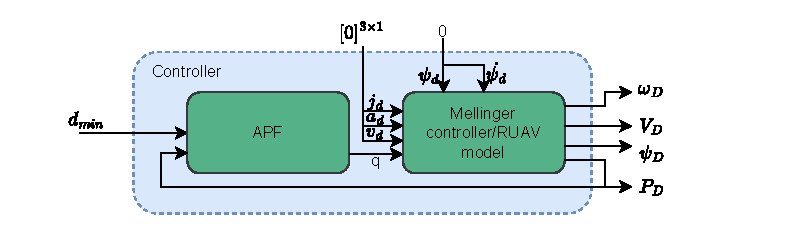
\includegraphics[width=\textwidth]{5-Figures/Chapter4/controller_architecture/APF_controller_architecture.pdf}
  \caption{outer/inner loop controller}
  \label{fig.4:APF_controller_architecture}
\end{figure}

\begin{figure}[htbp]
  \centering
  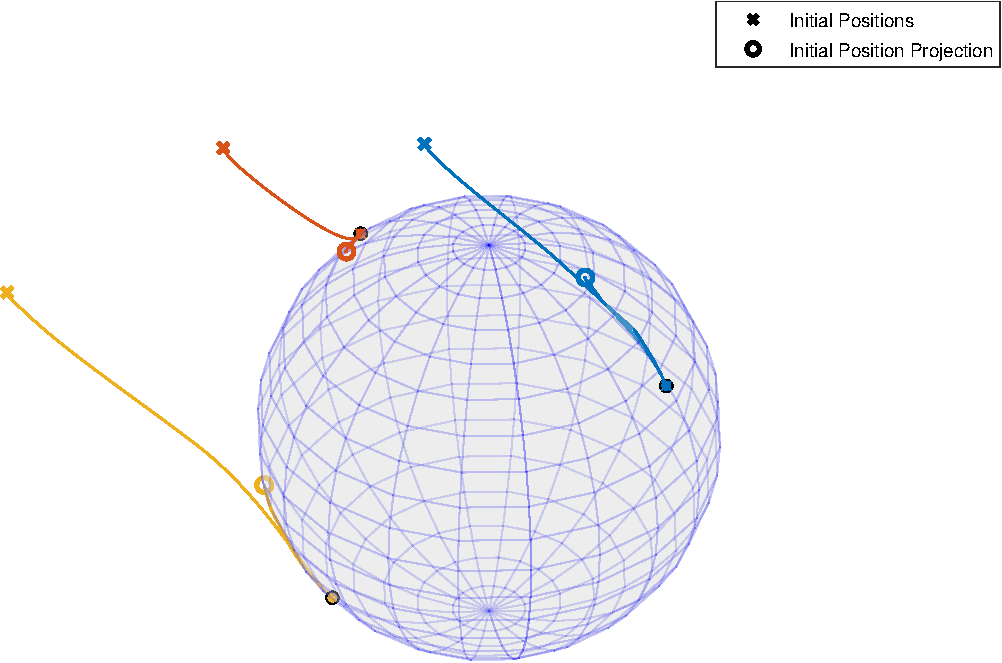
\includegraphics[width=0.8\textwidth]{5-Figures/Chapter4/solutions/APF.pdf}
  \caption{Trajectory obtained using the APF for three drones.}
  \label{fig.4:APF_solution}
\end{figure}

\subsection{Lyapunov control} \label{subsection.4:Lyapunov control}

Lyapunov controllers have been mentioned previously in Section \ref{sec.3:Lyapunov Stability and Lyapunov-Based Control}, not only the general introduction but the explicit controller to be used obtained from \cite{lyapunov_outer_loop_control}.This section describes the geometric  control architecture implementation in $\mathbb{S}^2$. As in the \gls{APF} approach, the Fibonacci lattice is first computed as a set of reference points $\{ \gls{p_i_desired} \in \mathbb{S}^2 \}_{i=1}^{N_D}$ distributed on a sphere of radius \gls{desired_sphere_radius}.

Using the Lyapunov-based control actuation defined in Section~\ref{sec.3:Lyapunov Stability and Lyapunov-Based Control} as the geometric controller and maintaining the internal Mellinger controller. In this geometric controller implementation the points \gls{q} are driven toward their corresponding target \gls{q_desired} with exponentially decreasing error.

The overall control architecture is shown in Figure~\ref{fig.4:Lyapunov_controller_architecture}, and the resulting system behavior is illustrated in Figure~\ref{fig.4:Layapunov_solution}. This formulation enables stable multi-agent motion constrained to a spherical surface while preserving geometric consistency and ensuring dynamic feasibility.

\begin{figure}[htbp]
  \centering
  \includegraphics[width=\textwidth]{5-Figures/Chapter4/controller_architecture/Lyapunov_controller_architecture.pdf}
  \caption{outer/inner loop controller}
  \label{fig.4:Lyapunov_controller_architecture}
\end{figure}

\begin{figure}[htbp]
  \centering
  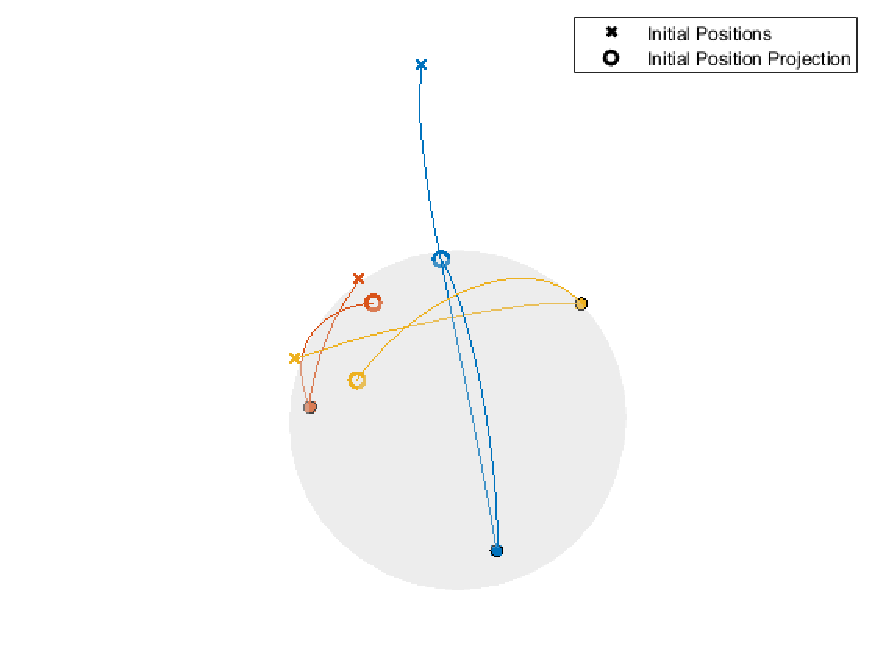
\includegraphics[width=0.8\textwidth]{5-Figures/Chapter4/solutions/lyapunov.pdf}
  \caption{Trajectory obtained using the Lyapunov for three drones.}
  \label{fig.4:Layapunov_solution}
\end{figure}

\subsection{Methods comparison} \label{sec.4:Methods comparison}

After analyzing all three methods, it was determined that the use of Lyapunov-based control is the most suitable choice for the intended purpose. This is due to its superior speed and precision compared to the other two studied approaches. With this controller defined, it is now possible to examine the remaining components of the system, beginning with the radius controller.

As illustrated in Figure~\ref{fig.4:Layapunov_solution}, there is no explicit control over the timing of the agents’ convergence to the target or the desired radius \gls{desired_sphere_radius}. Instead, the agents naturally converge to the waypoints \gls{q}, which are already located on the sphere defined by \gls{desired_sphere_radius}.

As will be discussed in the following section, the drone position \gls{chaser_pos} is first projected onto a sphere with a time-varying radius \gls{sphere_radius}, before ultimately converging to the desired radius \gls{desired_sphere_radius}.

\subsection{Radii control}

The goal of this controller is to change the value of the sphere radius \gls{sphere_radius} until it is the same as  \gls{desired_sphere_radius}, but it is not desired for the radius to simply modify as fast as possible to the desired value as it might be on some other controllers in this case the radius will only adjust when the drone \gls{chaser_pos} is radially located "above" the point \gls{p_desired} as well as the velocity of the chaser and target is the same or near the same. The objective of this controller can formally be defined by
\begin{equation*}
    \lim_{t \to \infty} \gls{ith_sphere_radius}(t) = \gls{desired_sphere_radius}, \forall i \in \mathbb{N}
\end{equation*}
Let the relative position and velocity between target and UAV be defined as
\begin{align}
    R_i = \gls{target_pos} - \gls{chaser_i_pos}, \quad v_i = \dot{p}_T - \dot{p}_i
\end{align}
and defining the radial direction as
\begin{equation}
    \hat{r}_i = \frac{R_i}{\|R_i\|}
\end{equation}
To avoid undesirable coupling between angular convergence and radial contraction, the relative velocity is decomposed into radial and tangential components, being the tangential component defined as
\begin{equation}
    v_{i\perp}
    =
    v_i - (v_i^\top \hat{r}_i)\hat{r}_i
\end{equation}
The reason for the radial component being neglected comes as a way to prevent feedback between radius reduction and radial acceleration, which would otherwise induce oscillatory behavior. 
It is then possible to define the adaptive law
\begin{equation}
\dot{r}_i = k_{\mathrm{rad}} e^{-( \|e_{q_i}\| + \|v_{i\perp}\| )^2}
\left( \gls{desired_sphere_radius} - \gls{ith_sphere_radius} \right)
\label{eq:new_radial_control}
\end{equation}
where $\gls{ith_sphere_radius} = \|\gls{chaser_i_pos} - \gls{target_pos}\|$ is the current encirclement radius, $e_{q_i}$ is the reduced-attitude error defined in \eqref{eq.3:new_err_ref_dynamic} and $k_{\mathrm{rad}} > 0$ is a constant scaler gain.

The exponential modulation term plays a key stabilizing role. 
When either the angular error $\|e_{q_i}\|$ or the tangential relative velocity $\|v_{i\perp}\|$ is large, the exponential term becomes small, effectively slowing radial contraction. 
This ensures that the directional alignment on $\Gamma^2$ is prioritized before aggressive radial motion happens. 

As $\|e_{q_i}\| \to 0$ and $\|v_{i\perp}\| \to 0$, the exponential term approaches unity, as can be seen in Figure~\ref{fig.4:radii_gain}, and the radius converges to $\gls{desired_sphere_radius}$.

\begin{figure}[t]
\centering
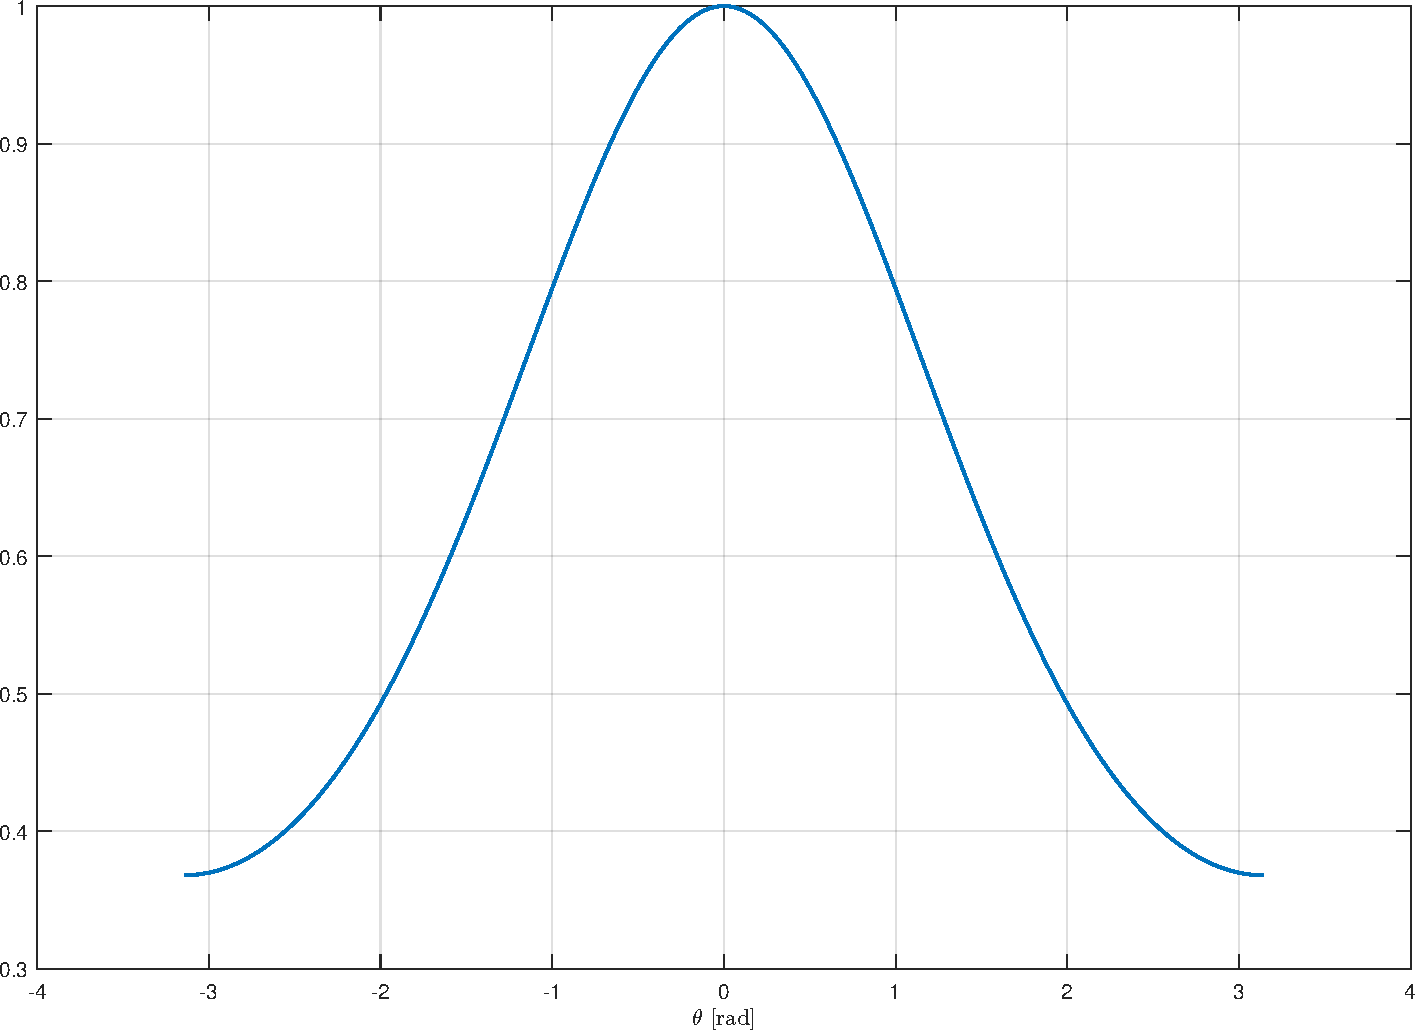
\includegraphics[width=0.85\columnwidth]{5-Figures/Chapter4/Radii/radii_gain.pdf}
\caption{Radial gain given displacement, ($v_{i\perp} = 0$)}
\label{fig.4:radii_gain}
\end{figure}

Consequently, from the control law given in the Lyapunov controller and Radii controller, it can be seen that
\begin{equation}
\lim_{t \to \infty} \gls{q_i}(t) = \gls{q_i_desired},
\quad
\lim_{t \to \infty} \gls{ith_sphere_radius}(t) = \gls{desired_sphere_radius}
\end{equation}
Thus, it is possible to formulate a controller that is capable of achieving the desired points in $\Gamma^2$ from any position in $\mathbb{R}^3$ implying
\begin{equation}
\lim_{t \to \infty} \gls{chaser_i_pos}(t) = \gls{target_pos} + \gls{desired_sphere_radius} \gls{q_i_desired} = \gls{p_i_desired}.
\end{equation}

In Figure~\ref{fig.4:Layapunov_and_radii} it is possible to see two circles the current radius \gls{sphere_radius} the drone is encircling the target with, in blue, and the final desired radii \gls{desired_sphere_radius} that all agents must get to, in red. In Figure~\ref{fig.4:radii_evolution_in_time} is is possible to see the intra distance of the agent and the target over the entire simulation period of time.

\begin{figure}[htbp]
  \centering
  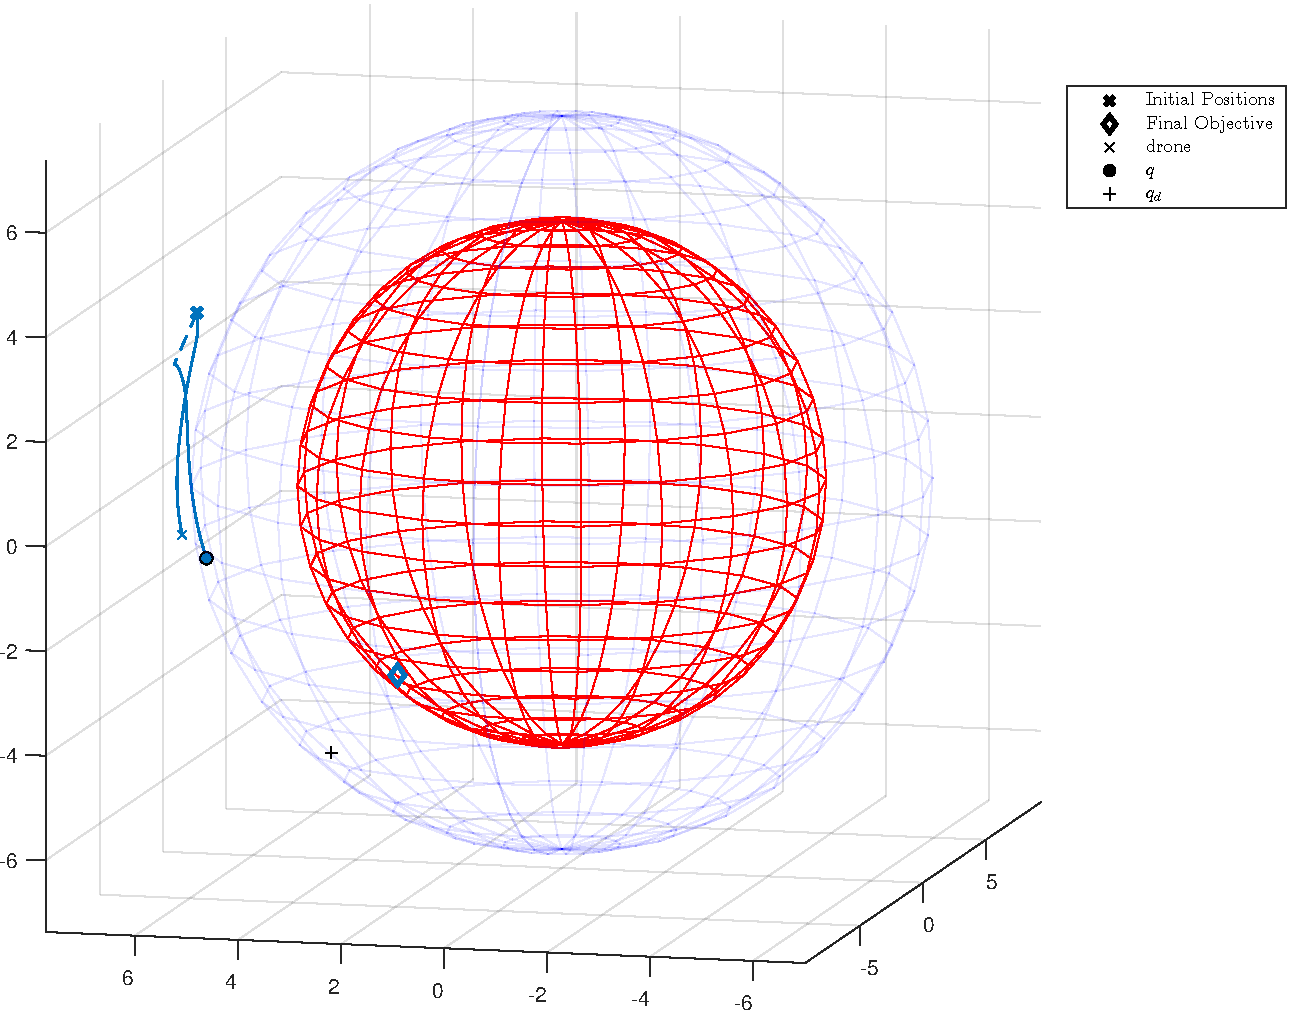
\includegraphics[width=0.8\textwidth]{5-Figures/Chapter4/Radii/lyapunov_radii.pdf}
  \caption{Trajectory obtained for 1 drone mid simulation.}
  \label{fig.4:Layapunov_and_radii}
\end{figure}

\begin{figure}[htbp]
  \centering
  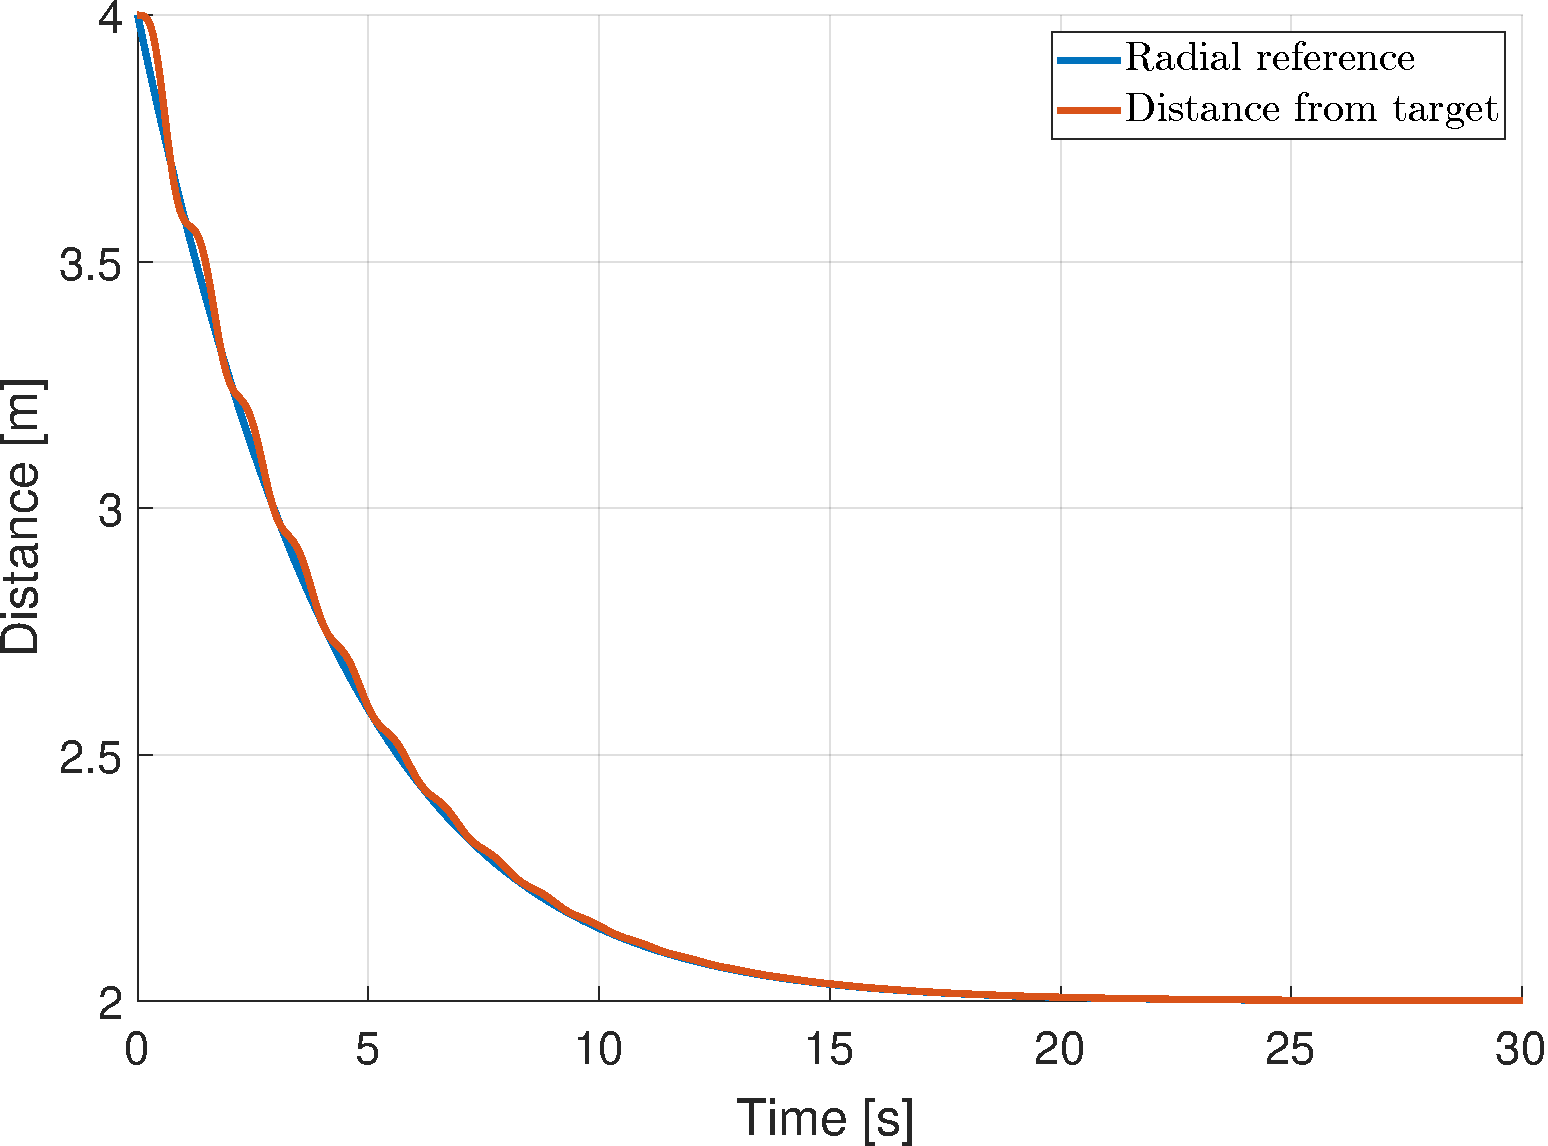
\includegraphics[width=0.8\textwidth]{5-Figures/Chapter4/Radii/radiii_distance.pdf}
  \caption{Intra distance between agent and target}
  \label{fig.4:radii_evolution_in_time}
\end{figure}

It was also implemented that instead of moving each agent toward a randomly selected Fibonacci point on the sphere, the drones are assigned to target points using the Munkres algorithm. Given a cost matrix defined as the geodesic distance between each drone and all target points projected onto the final-radius sphere \gls{desired_sphere_radius}, the algorithm computes an optimal solution to the \gls{GNN} assignment problem. This solution minimizes the total assignment cost. No custom implementation of the algorithm was developed, instead, the built-in \(\text{MATLAB}^\text{\textregistered}\) \cite{MATLAB:R2024a} function \textit{assignmunkres} \cite{MATLAB_assignmunkres} was used.

\section{Safe Guard Artificial Potential Fields}

Although the introduction of the radii controller improves tracking of the Lyapunov-based controller, it does not guarantee collision avoidance between agents as they move toward their assigned Fibonacci lattice points. To enhance system safety, an \gls{APF} is introduced to generate repulsive effects on the reference positions, preventing inter-agent collisions during transients.

The \gls{APF} is applied at the reference level rather than directly at the actuation level. This design choice increases modularity and preserves the structure of the low-level controller, keeping it decoupled from higher-level coordination strategies. Furthermore, given the presence of the radii controller and appropriately tuned gains, each \gls{UAV} is assumed to accurately track its reference, resulting in minimal deviation between desired and actual positions.

The safeguard operates directly on the spherical manifold $\Gamma^2$ and modifies only the reference position $\gls{q_i}$, preserving the nonlinear controller stability and Lyapunov convergence properties. At each control step, the current \gls{UAV} positions are projected onto the sphere of radius \gls{desired_sphere_radius} centered at the target:
\begin{equation}
    q_{i}^{\gls{desired_sphere_radius}} = \Pi_{\Gamma^2}^{\gls{desired_sphere_radius},\gls{target_pos}}(\gls{q}).
\end{equation}

Pairwise geodesic distances on $\Gamma^2$ are then computed. Let $d_{ij}$ denote the spherical geodesic distance between UAVs $i$ and $j$. A minimum safe separation $\gls{min_dist} > 0$ is defined, chosen here as half of the average geodesic distance between the desired Fibonacci configuration points $p^\star$. For each neighboring \gls{UAV} satisfying $d_{ij} < \gls{min_dist}$, a repulsive tangential displacement is generated. Equation~\eqref{eq.4:radial_direction} denotes the outward normal direction at \gls{target_pos}.
\begin{equation}
    n_i = \frac{q_{i}^{\gls{desired_sphere_radius}} - \gls{target_pos}}{\|q_{i}^{\gls{desired_sphere_radius}} - \gls{target_pos}\|}
    \label{eq.4:radial_direction}
\end{equation} 
The relative displacement vector given by
\begin{equation}
    \Delta_{ij} = q_{i}^{\gls{desired_sphere_radius}} - q_{j}^{\gls{desired_sphere_radius}}
\end{equation}
is decomposed into radial and tangential components. Only the tangential component
\begin{equation}
    \Delta_{ij}^{\top}
    =
    \Delta_{ij}
    -
    (\Delta_{ij}^{\top} n_i)\, n_i
\end{equation}
is retained, ensuring that the safeguard does not interfere with radial stabilization. The repulsive contribution from agent $j$ to agent $i$ is defined as
\begin{equation}
    f_{ij}
    =
    (\gls{min_dist} - d_{ij})
    \frac{\Delta_{ij}^{\top}}{\|\Delta_{ij}^{\top}\|}
\end{equation}
if $d_{ij} < \gls{min_dist}$ and zero otherwise. The total artificial potential displacement is obtained by summing all active pairwise contributions:
\begin{equation}
    f_i = \sum_{j \neq i} f_{ij}.
\end{equation}
To prevent excessive deviation from the nominal reference, the resulting displacement is saturated to a bounded magnitude (at most \gls{min_dist}), and the corrected reference is re-projected onto the sphere:
\begin{equation}
    \tilde{q}_i =
    \Pi_{\Gamma^2}^{\gls{desired_sphere_radius},\gls{target_pos}}
    \left(
        q_{i}^{\gls{desired_sphere_radius}} + f_i
    \right).
    \label{eq:apf_result}
\end{equation}
The safeguard therefore produces a modified reference direction $\tilde{q}_i$ that maintains spherical consistency while enforcing minimum separation during transients.

\paragraph*{Stability Discussion}

The \gls{APF} term acts as a bounded perturbation to the nominal reduced-attitude reference. Since the artificial potential vanishes whenever $d_{ij} \ge \gls{min_dist}$ for all $j$, the nominal equilibrium configuration remains unchanged. Furthermore, because the perturbation is tangential and bounded, the almost-global asymptotic stability of the reduced-attitude equilibrium is preserved in the sense of input-to-state stability with respect to the safeguard perturbation.

In practice, this mechanism improves safety during convergence by reducing the likelihood of collisions, while allowing the Lyapunov-based controller to recover the desired encirclement configuration once agents are sufficiently separated. However, unlike \gls{CBF}, this method does not provide formal collision avoidance guarantees.

\section{Consensus}

Consensus has been thoroughly referenced and explained in Section~\ref{sec.3:Consensus-Based Coordination}, here and from now on unlike the previous chapter examples the target exact position is unknown and the same might also be in motion. Since in practice, each agent only has access to its own noisy measurements. A fully connected consensus algorithm is employed, allowing all agents to share information and estimate the target position collectively.

Due to the fully connected communication graph, the consensus process converges to the average of the individual measurements. To account for the dynamic nature of the moving target an exponential moving average, referenced in Section~\ref{sec.3:Exponential Moving Average} is used, enabling the estimate to adapt to new measurements while filtering out noise.

In Figure~\ref{fig.4:Consensus between 3 agents of target position} its possible to see the target motion as well as the target estimation, it is also possible to see that the 3 targets reach the same or near same value for the position of the target as is expected. Note that non of the lines represent agents only the estimated position of the target given by each one of them.

\begin{figure}[htbp]
  \centering
  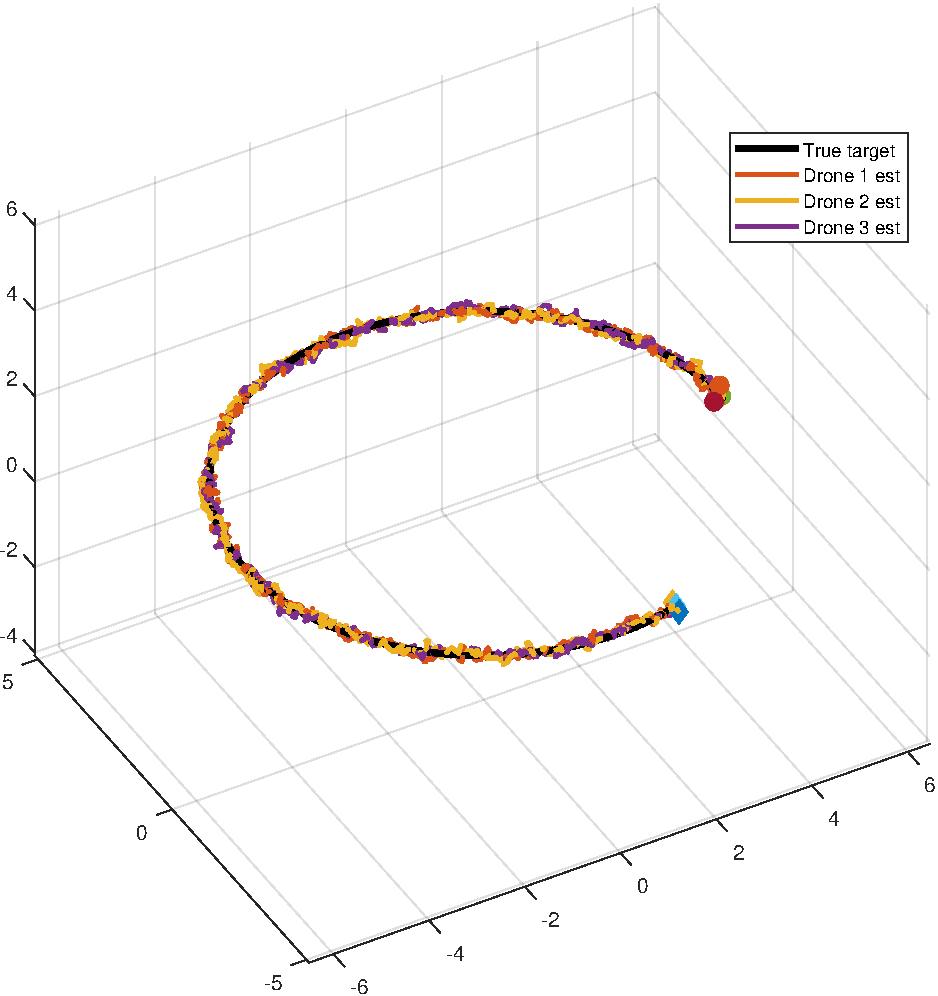
\includegraphics[width=0.8\textwidth]{5-Figures/Chapter4/Consensus/moving_target_consensus.pdf}
  \caption{Consensus between 3 agents of target position}
  \label{fig.4:Consensus between 3 agents of target position}
\end{figure}

% ===================== Simulation Results =====================
\section{Simulation Results} \label{sec.4:simulations}

Two encirclement scenarios are tested in simulation, considering only 3 drones for simplicity of visualization, first a simulation with a stationary target and second, one where the target moves. 
The results are shown in Figures~\ref{fig.4:results_drone_1_stationary}, \ref{fig.4:lyapunov_solution_stationary} for a stationary target and \ref{fig.4:results_drone_1} and \ref{fig.4:lyapunov_solution_t_0.5}--\ref{fig.4:lyapunov_solution_t_30} for a moving one. 
The parameters using are reported in Table~\ref{tab.4:all_params} and the initial positions of the drones are defined in Table~\ref{tab.4:Drone_positions}.The target reference position $\gls{target_pos}^\star$ was defined by the piecewise trajectory defined in Equation~\eqref{eq.4:sim_target_motion} being the target nonlinear controller and dynamics the same as the chasers (Table: \ref{tab.4:all_params}). As noted in~\cite{mycielskiTheoriesPursuitEvasion1988}, independently of implementation in order to encircle or capture a target the chasers need to possess a maximum velocity not lower than that of the target, in this case since the model is the same, both target and chasers achieve the same maximal velocity.

\begin{table}[htbp]
    \centering
    \caption{Simulation and Control Parameters}
    \label{tab.4:all_params}
    \begin{tabular}{l c}
    \hline
    \textbf{Parameter} & \textbf{Value} \\
    \hline
    \multicolumn{2}{c}{\textit{General Simulation Parameters}} \\
    \hline
    Simulation duration $T_{\mathrm{end}}$ & $30~\mathrm{s}$ \\
    Sampling period $\Delta t$ & $0.01~\mathrm{s}$ \\
    Gravity $g$ & $9.81~\mathrm{m/s^2}$ \\
    Number of drones $n_D$ & $3$ \\
    Desired sphere radius $\gls{desired_sphere_radius}$ & $2~\mathrm{m}$ \\
    Radial gain $K_{\mathrm{rad}}$ & $0.3$ \\
    \hline
    \multicolumn{2}{c}{\textit{Geometric Controller Parameters}} \\
    \hline
    Damping coefficient $c$ & $0.3$ \\
    Inertia matrix $I_q$ & $\mathrm{diag}(0.0294,\;0.0305,\;0.0495)$ \\
    Additional torques $\tau$ & $\mathbf{0}_{3\times1}$ \\
    Position gain $k_r$ & $70$ \\
    Angular velocity gain $k_\omega$ & $0.7056$ \\
    \hline
    \multicolumn{2}{c}{\textit{Consensus and measurement}} \\
    \hline
    EMA $\alpha_\text{EMA}$ & 0.2\\
    Measurement noise  & 0.05\\
    \hline
    \multicolumn{2}{c}{\textit{Nonlinear Controller Parameters}} \\
    \hline
    Mass $m_D$ & $5~\mathrm{kg}$ \\
    Inertia matrix $I_D$ & $\mathrm{diag}(0.02,\;0.02,\;0.03)$ \\
    Drag coefficient $D$ & $0$ \\
    Proportional gain $K_p$ & $\mathrm{diag}(150,\;150,\;150)$ \\
    Velocity gain $K_v$ & $\mathrm{diag}(15,\;15,\;15)$ \\
    Integral gain $K_i$ & $\mathbf{0}_{3\times3}$ \\
    Attitude gain $k_r$ & $\mathrm{diag}(8,\;8,\;8)$ \\
    Angular rate gain $K_\Omega$ & $\mathrm{diag}(0.5,\;0.5,\;0.5)$ \\
    \hline
    \end{tabular}
\end{table}

\begin{table}[htbp]
    \centering
    \caption{Drone Cartesian Positions}
    \begin{tabular}{l c} 
    \textbf{Drone} & \textbf{Position [x, y, z]} \\ \hline
    Drone 1 & $\begin{bmatrix} 0.0906 & 1.7572 & 1.1440 \end{bmatrix}$ \\
    Drone 2 & $\begin{bmatrix} 3.0407 & 6.8319 & 8.4783 \end{bmatrix}$ \\
    Drone 3 & $\begin{bmatrix} 7.4084 & 7.6290 & 3.8924 \end{bmatrix}$ \\
    \end{tabular}
    \label{tab.4:Drone_positions}
\end{table}

\begin{equation}
    \gls{target_pos}^\star =
    \begin{cases}
    \begin{bmatrix}
    2\sin\left(\dfrac{\pi t}{8}\right) &
    2\cos\left(\dfrac{\pi t}{8}\right) &
    1.5
    \end{bmatrix}^\top,
    & t \le 8 \\[12pt]
    \begin{bmatrix}
    0 &
    -2 &
    1.5
    \end{bmatrix}^\top,
    & t > 8 .
    \end{cases}
    \label{eq.4:sim_target_motion}
\end{equation}

It can be seen that in both cases the proposed control strategy successfully achieves encirclement of the target at the desired radius, while maintaining well-separated trajectories during convergence.

\begin{figure}[htbp]
    \centering
    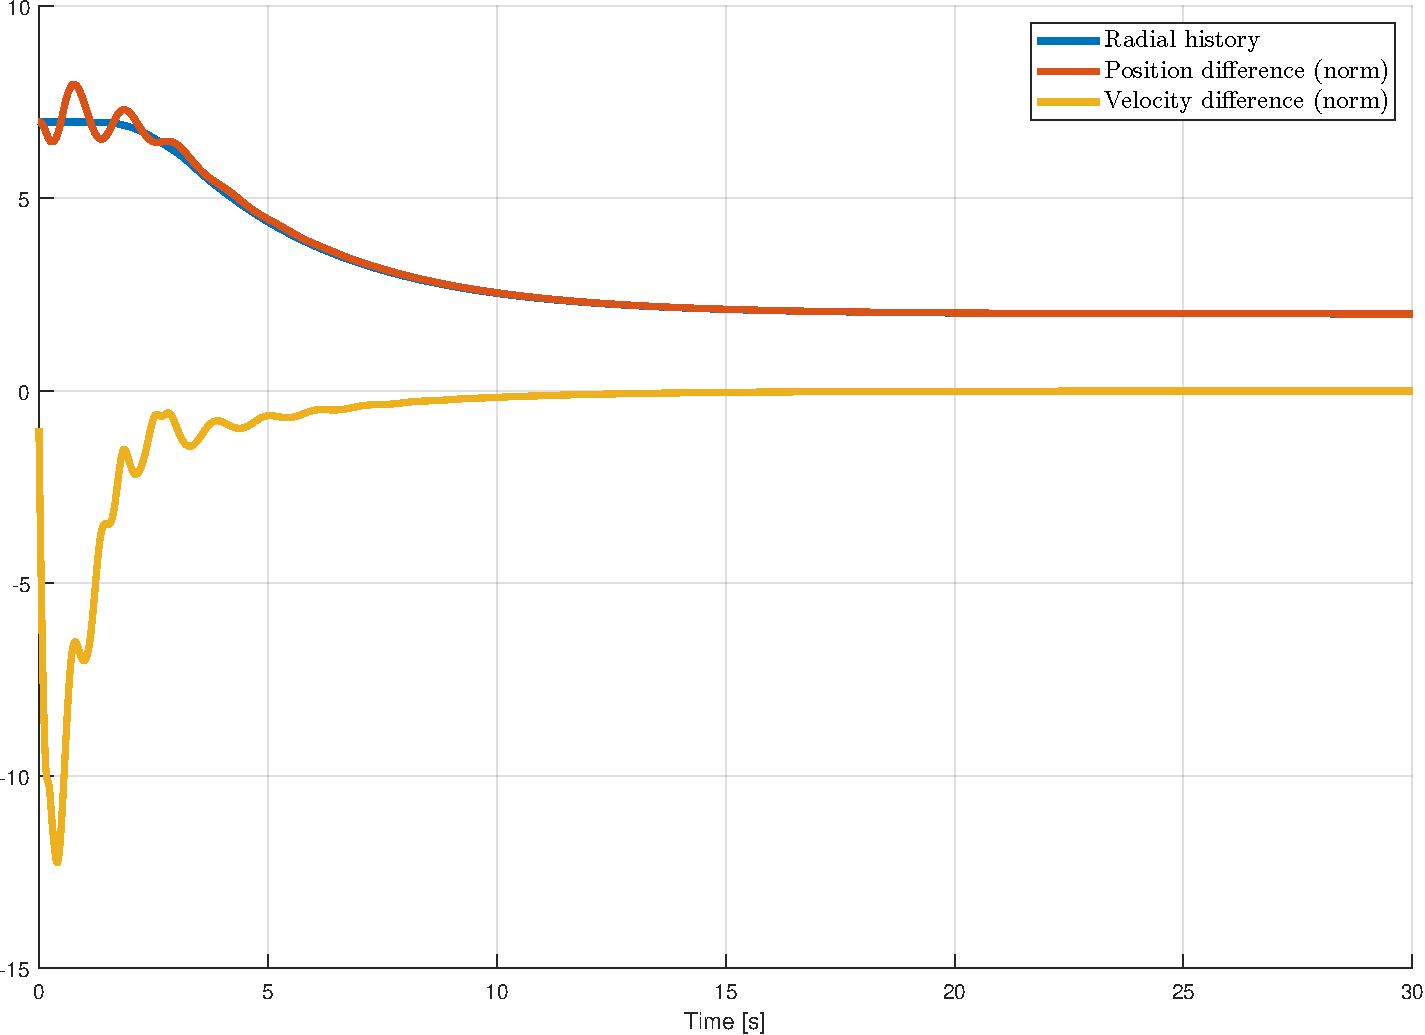
\includegraphics[width=0.85\columnwidth]{5-Figures/Chapter4/Final_Simulation/results_drone_1_stationary.pdf}
    \caption{Distance and velocity between drone 1 and a stationary target}
    \label{fig.4:results_drone_1_stationary}
\end{figure}

\begin{figure}[htbp]
    \centering
    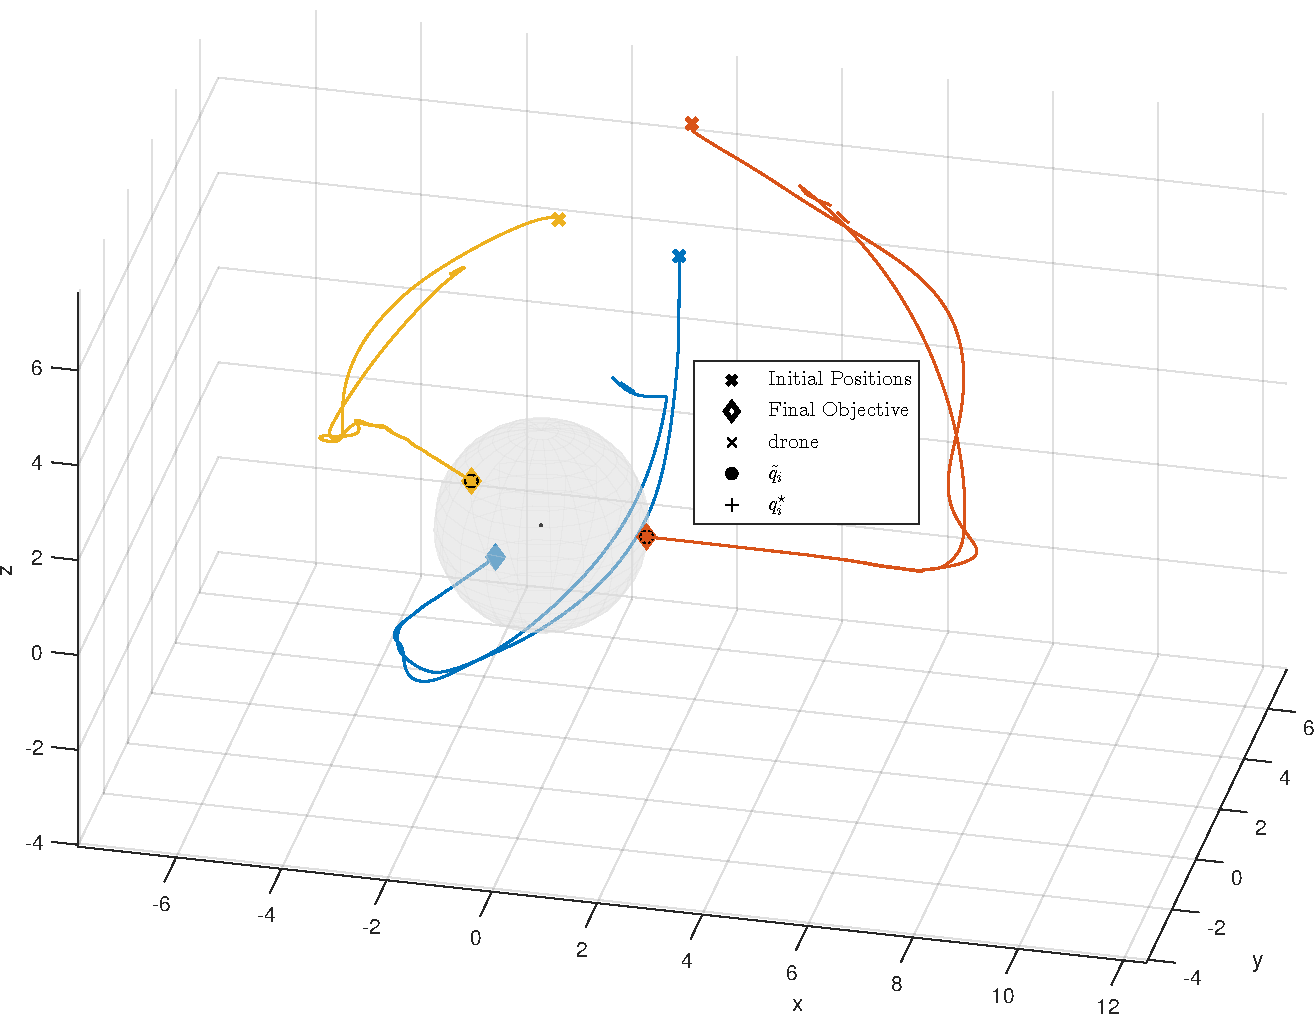
\includegraphics[width=0.85\columnwidth]{5-Figures/Chapter4/Final_Simulation/final_result_t_30_stationary.pdf}
    \caption{Encirclement of a stationary target using the Lyapunov-based control strategy for three drones after 30 seconds.}
    \label{fig.4:lyapunov_solution_stationary}
\end{figure}

\begin{figure}[htbp]
    \centering
    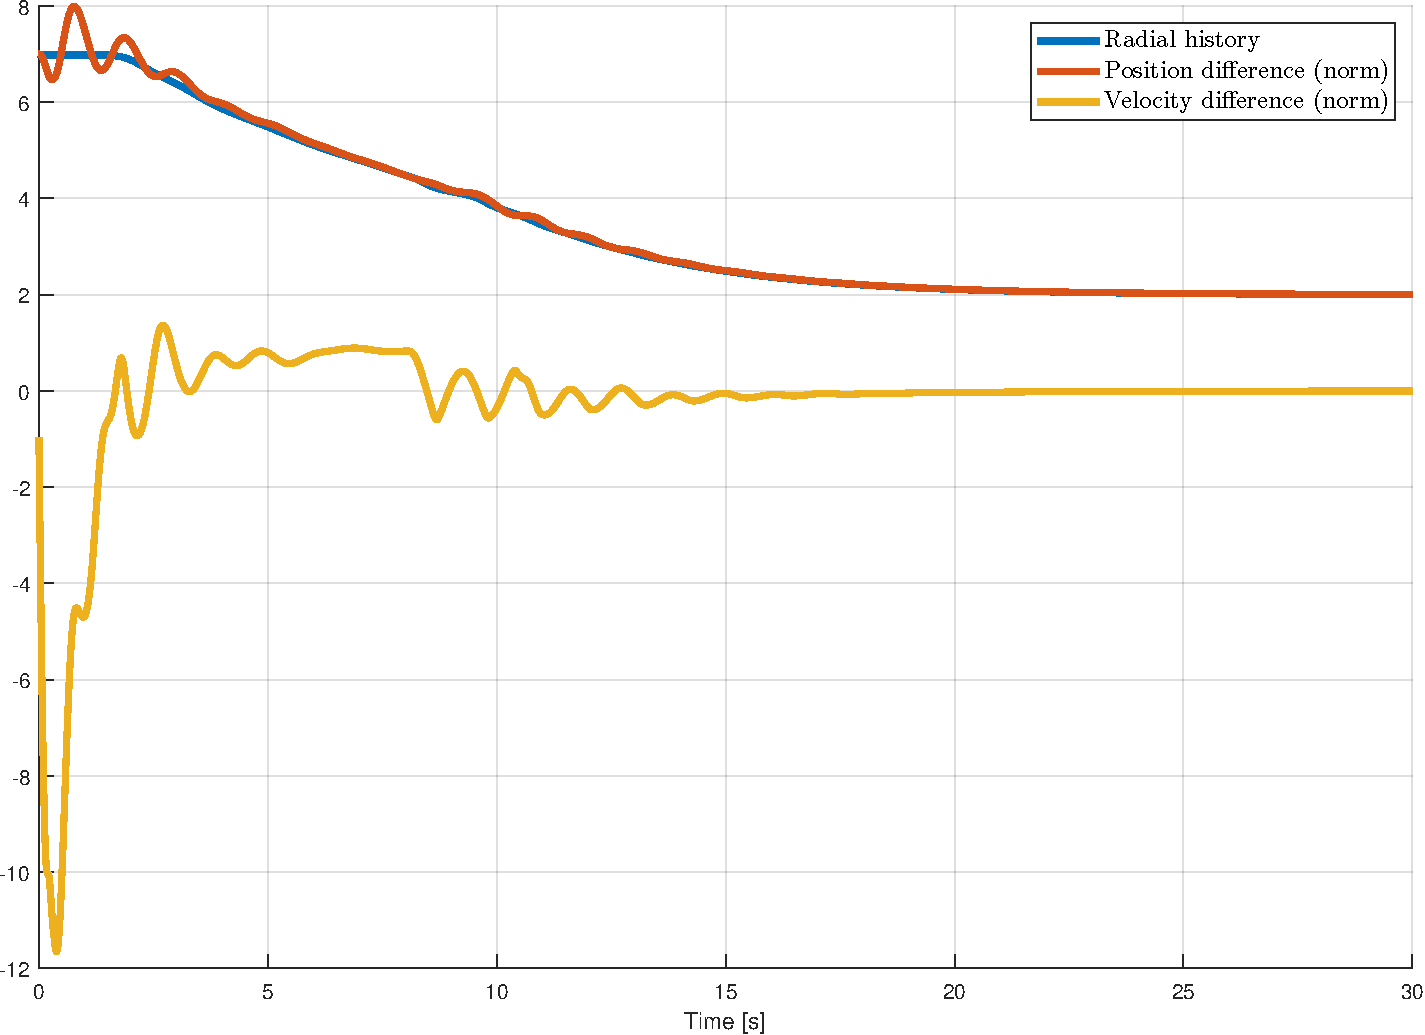
\includegraphics[width=0.85\columnwidth]{5-Figures/Chapter4/Final_Simulation/results_drone_1.pdf}
    \caption{Distance and velocity between drone 1 and a moving target}
    \label{fig.4:results_drone_1}
\end{figure}

\begin{figure}[htbp]
    \centering
    \subfloat[$t=0.5~\mathrm{s}$]{%
        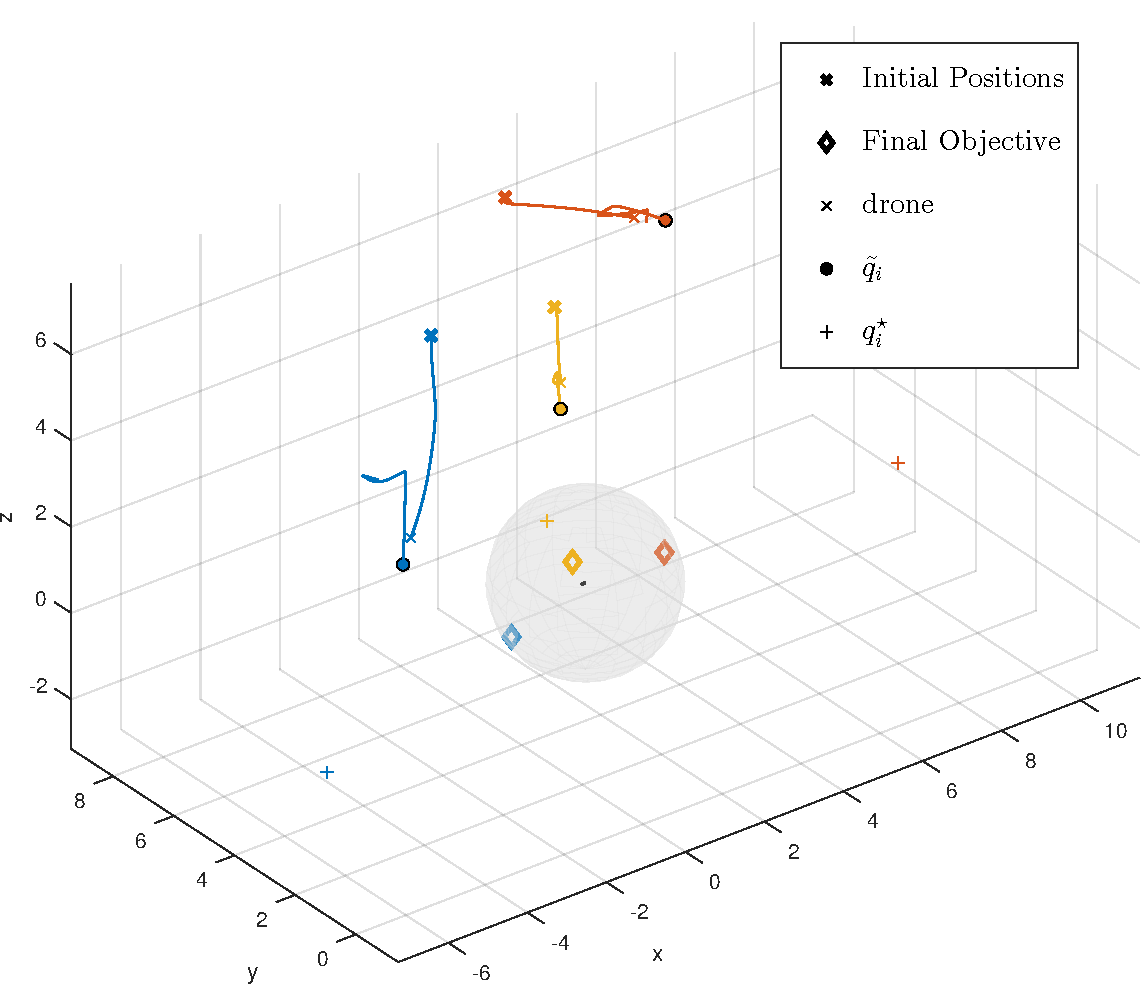
\includegraphics[width=0.5\columnwidth]{5-Figures/Chapter4/Final_Simulation/final_result_t_0.5.pdf}\hfil
        \label{fig.4:lyapunov_solution_t_0.5}
    }
        \subfloat[$t=3~\mathrm{s}$]{%
        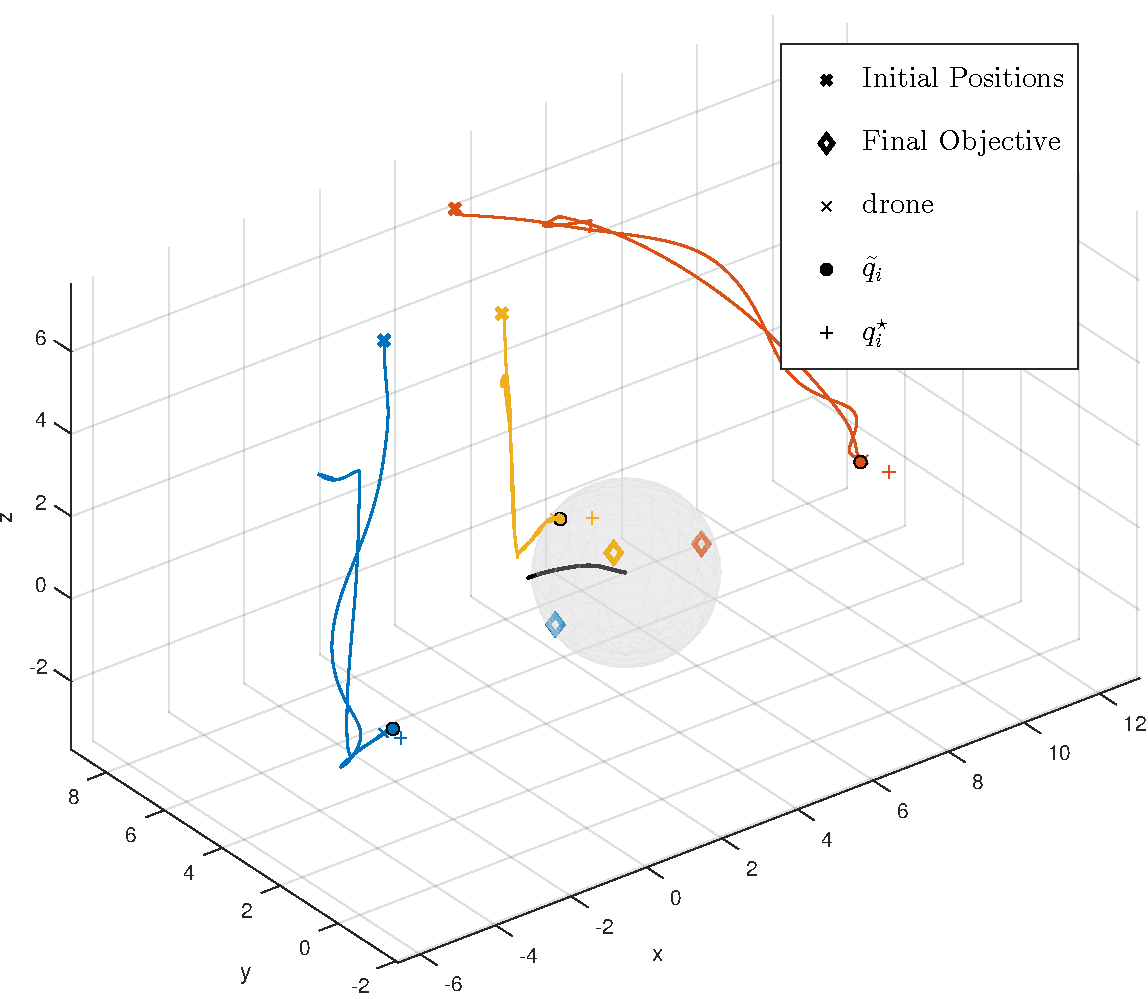
\includegraphics[width=0.5\columnwidth]{5-Figures/Chapter4/Final_Simulation/final_result_t_3.pdf}\hfil
        \label{fig.4:lyapunov_solution_t_3}
    }\\
    \subfloat[$t=6~\mathrm{s}$]{%
        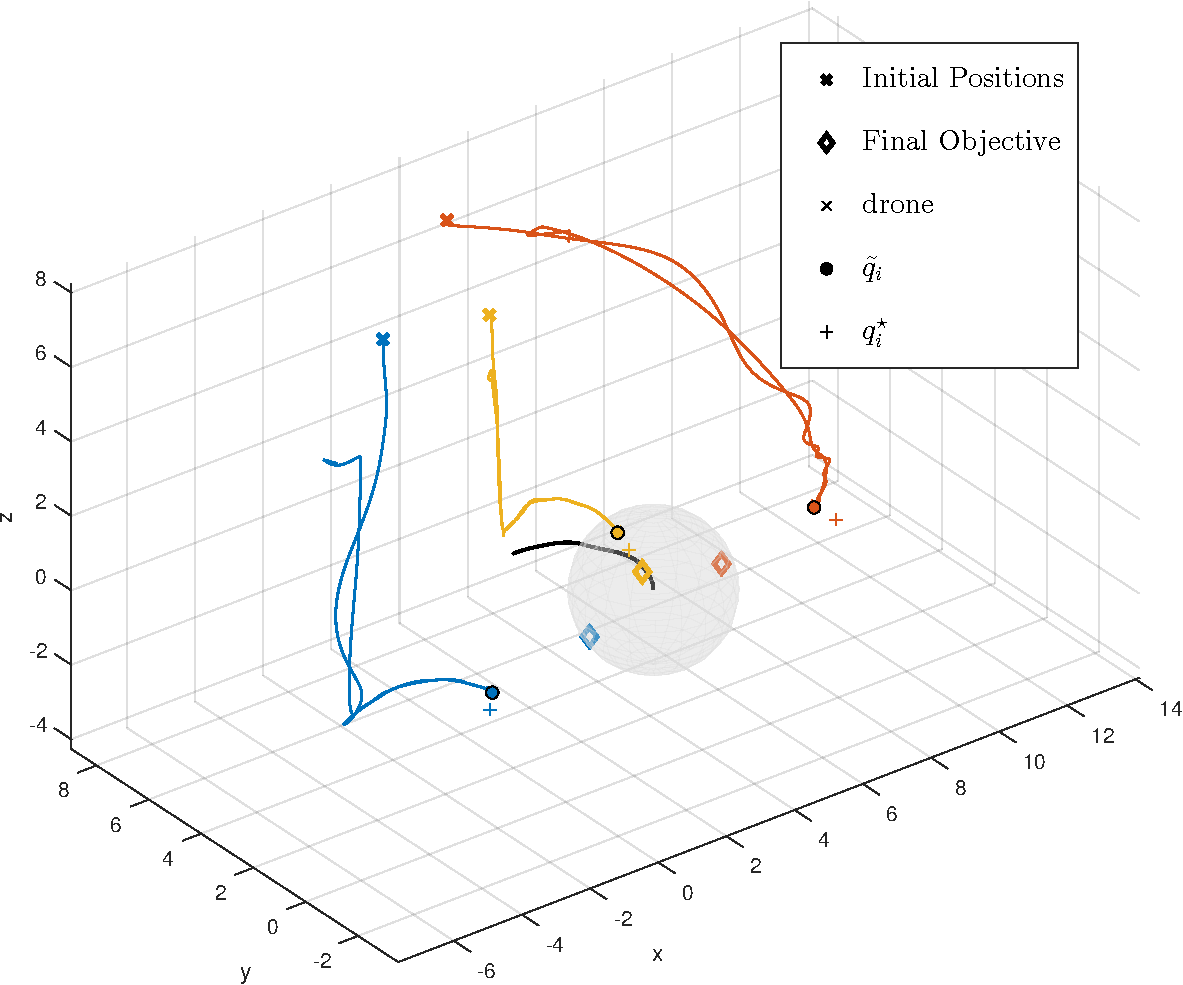
\includegraphics[width=0.5\columnwidth]{5-Figures/Chapter4/Final_Simulation/final_result_t_6.pdf}\hfil
        \label{fig.4:lyapunov_solution_t_6}
    }
    \subfloat[$t=30~\mathrm{s}$]{%
        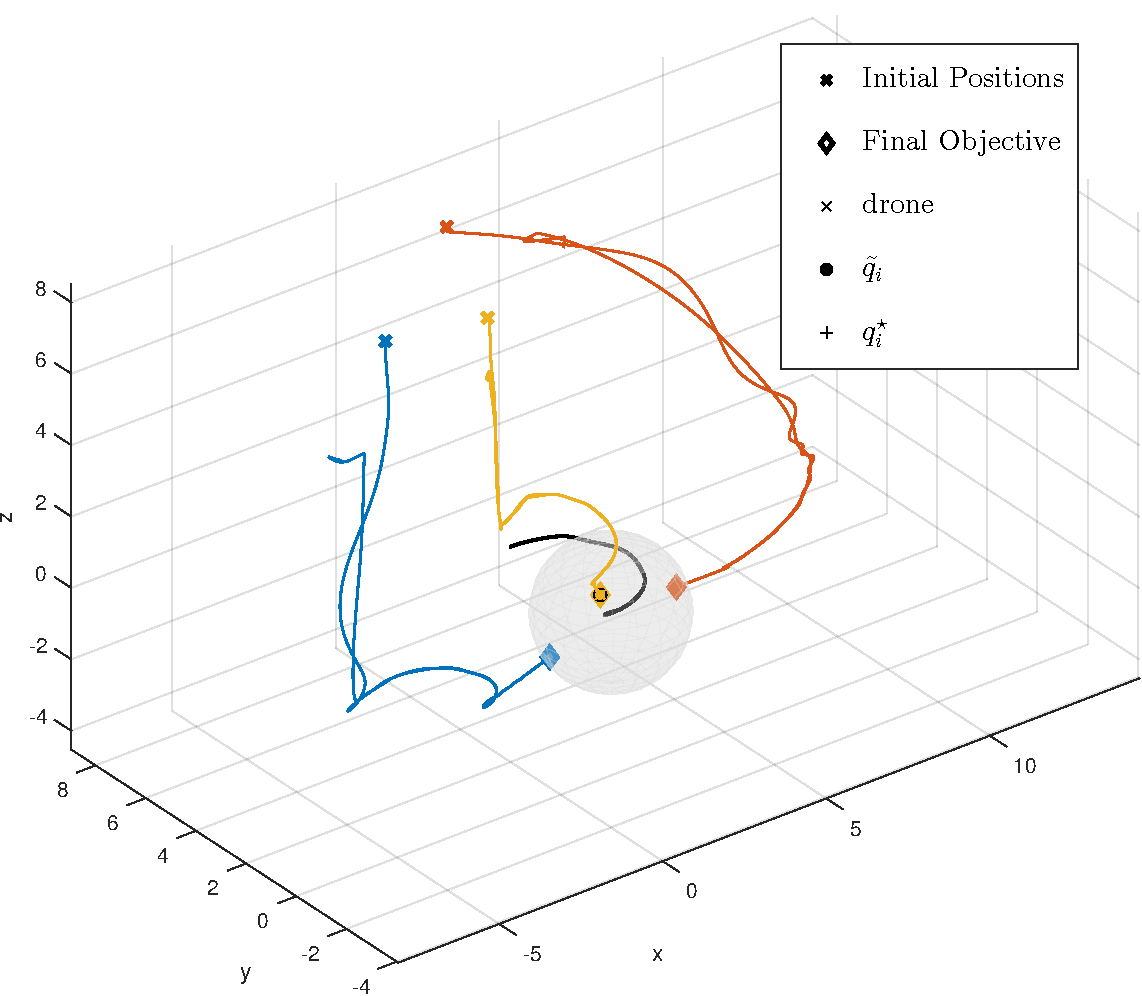
\includegraphics[width=0.5\columnwidth]{5-Figures/Chapter4/Final_Simulation/final_result_t_30.pdf}
        \label{fig.4:lyapunov_solution_t_30}
    }
    \caption{Encirclement of a moving target using the Lyapunov-based control strategy for three drones at different time instants.}
    \label{fig.4:lyapunov_solution}
\end{figure}